\section{\Glsfmtlong{MLTB}}\label{sec:b}
\setlength{\epigraphwidth}{\textwidth}
\epigraph{\small "Thinking, analyzing, inventing are not anomalous acts, they are the normal breathing of intelligence. To glorify the occasional fulfillment of that function, to treasure old and foreign thoughts, to recall with incredulous amazement what the doctor universalis thought, is to confess our languor or our barbarism. Every man must be capable of all ideas, and I understand that in the future he will be."}{"Pierre Menard, author of Don Quixote", "Ficciones", Jorge Luis Borges}


Throughout these four months, POKTscan and PNYX have worked on reproducing the \gls{HFOLML} \cite{noauthor_open_nodate} that serves as a reference for the Pocket Network community. 
All the code for reproduction is available in the repository. 
This conclude our series of reports, that has to be considered as a whole to understand the full picture of the work done. 
Throughout this section we will summarize the different modules:

\begin{itemize}[noitemsep]
    \item \textbf{Manager}
    \item \textbf{Regisrter}
    \item \textbf{Sampler}
    \item \textbf{Requester}
    \item \textbf{Evaluator}
\end{itemize}

and how they they interact, as detailed from Figure \ref{secb:fig:wf1} to \ref{secb:fig:wf9}. 
It is important to mention that we will not delve into some of the design decisions that were made, since most of these were discussed in the previous reports \footnote{\url{https://github.com/pokt-scan/pocket-ml-testbench/tree/main/reports}}, which we refer the reader to for more details. 
Finally, the results obtained when evaluating some \glspl{LM} will be presented.  

\begin{figure}[H]
    \centering        
    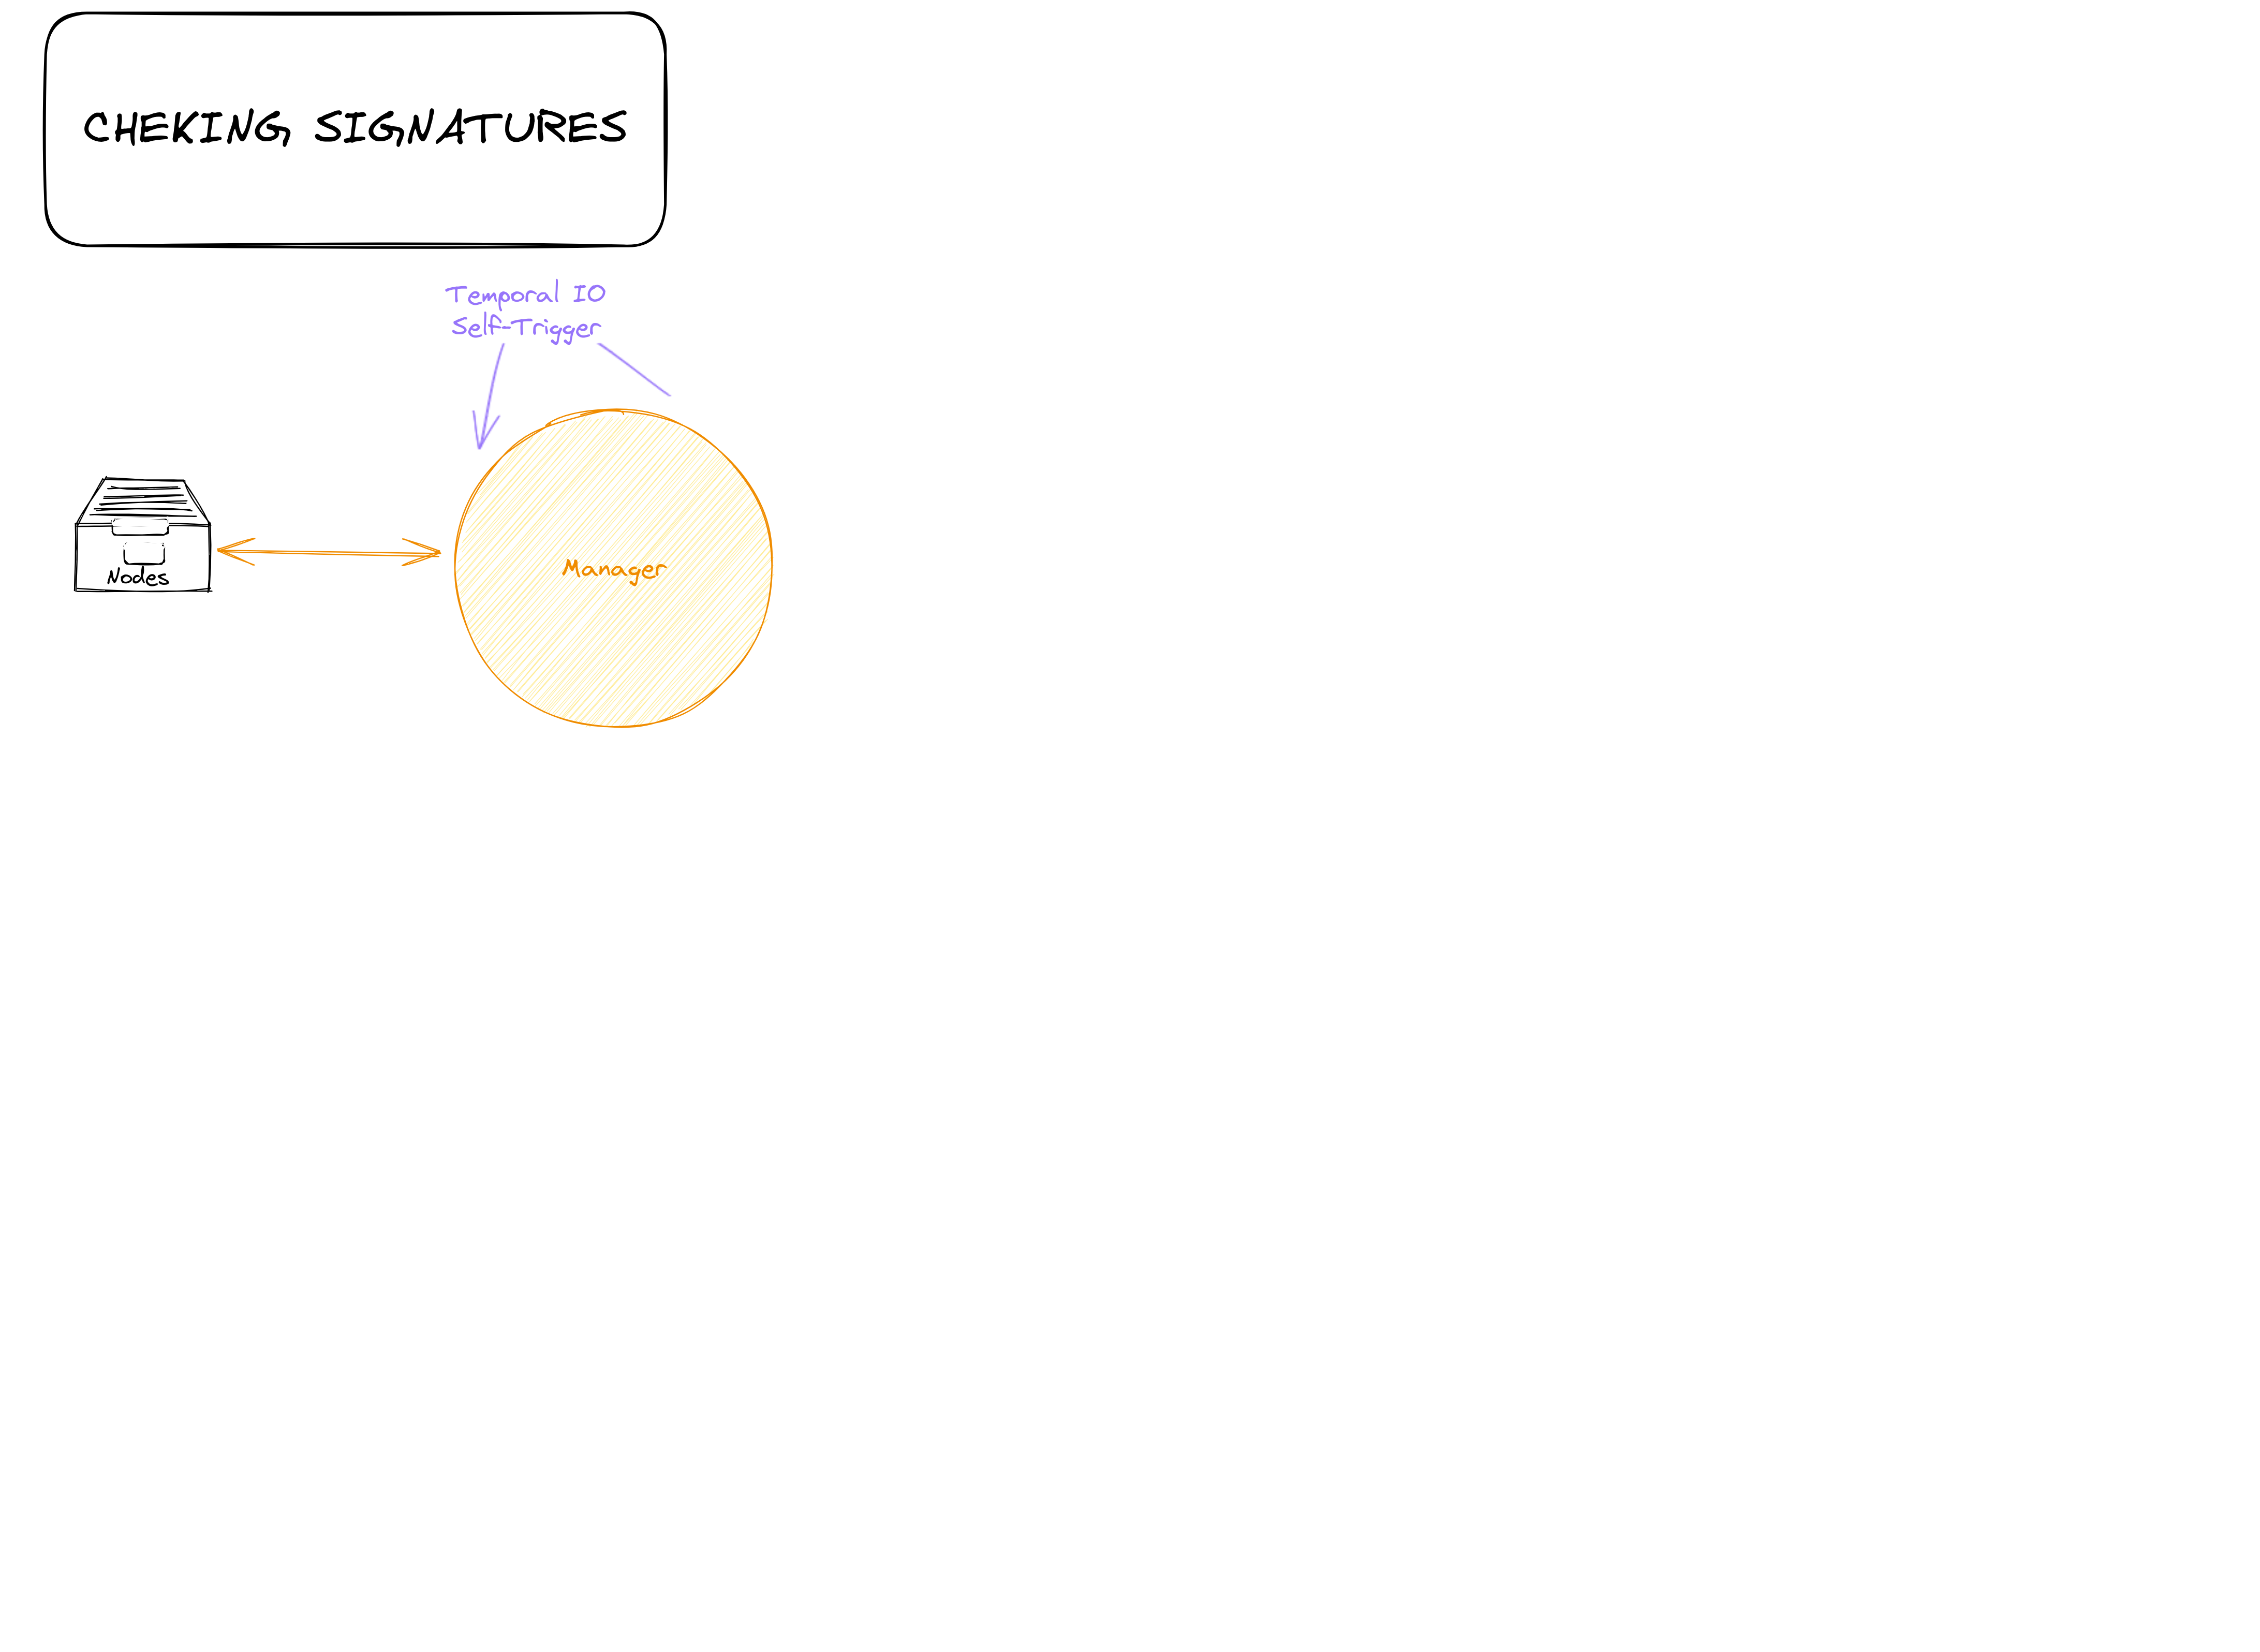
\includegraphics[width=0.8\textwidth]{workflow1}
    \caption{}
    \label{secb:fig:wf1}
\end{figure}

\begin{figure}[H]

    \centering        
    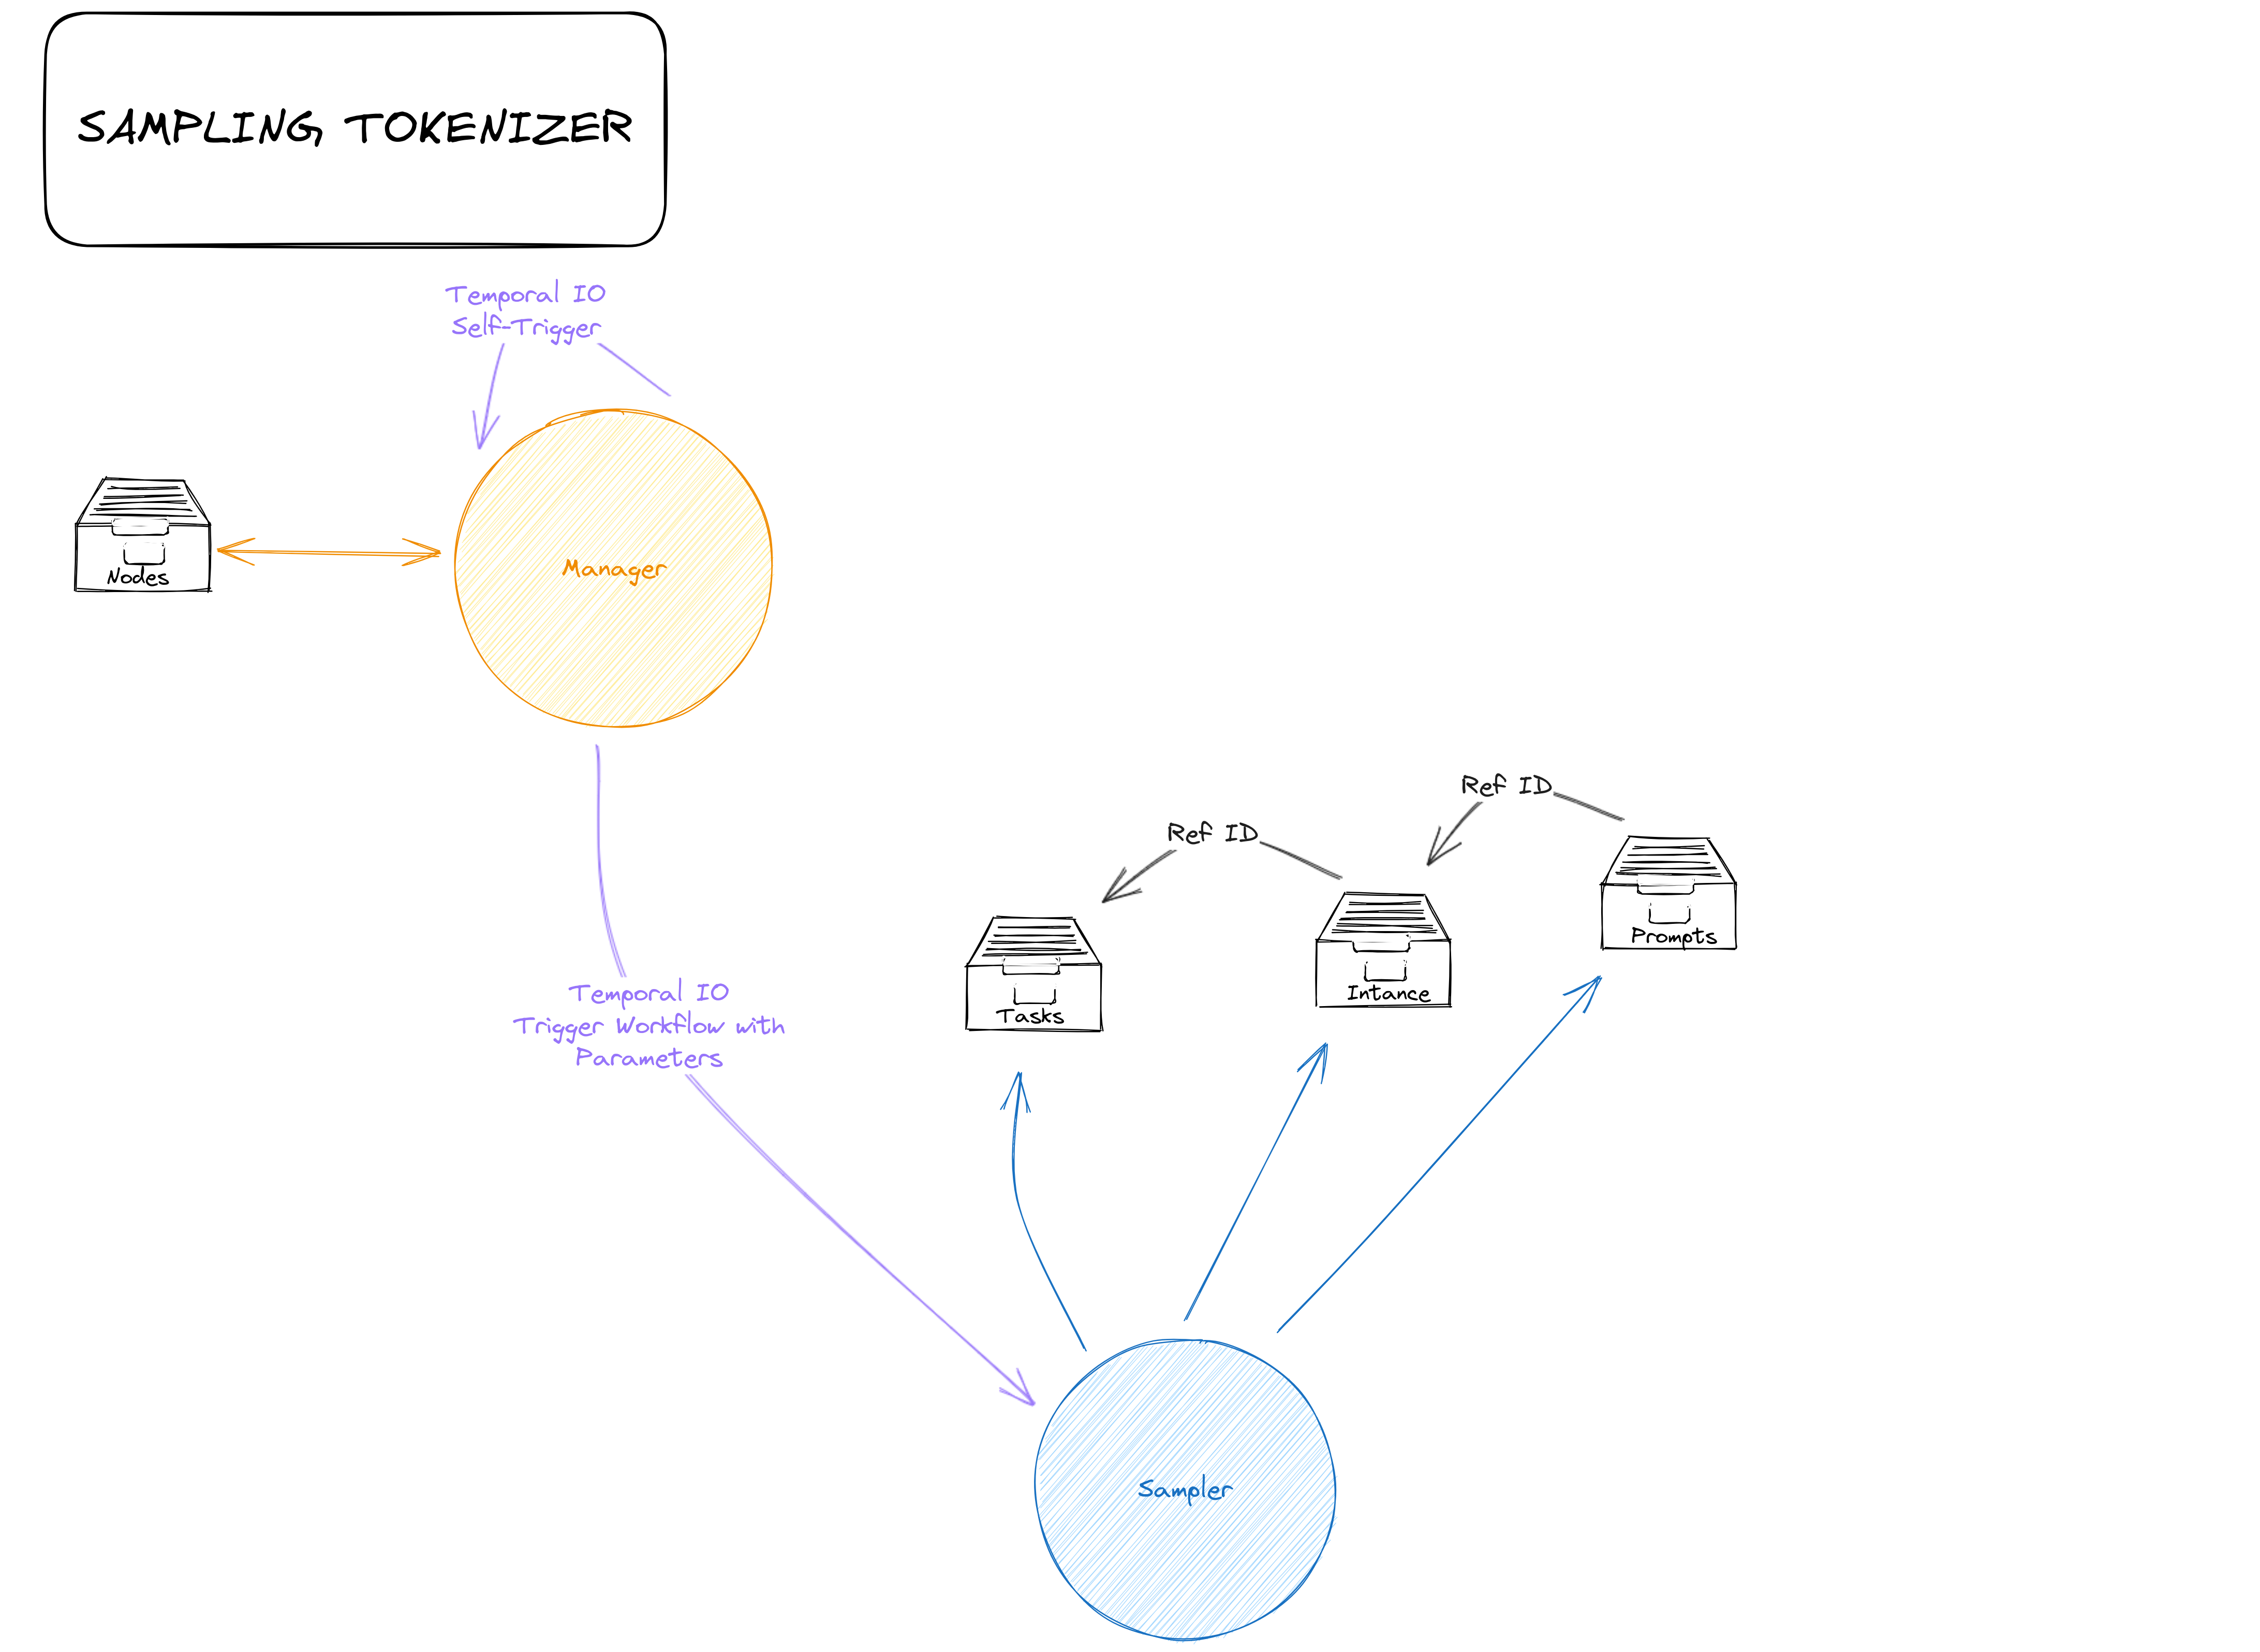
\includegraphics[width=0.8\textwidth]{workflow2}
    \caption{}
    \label{secb:fig:wf2}
\end{figure}

\begin{figure}[H]
    \centering        
    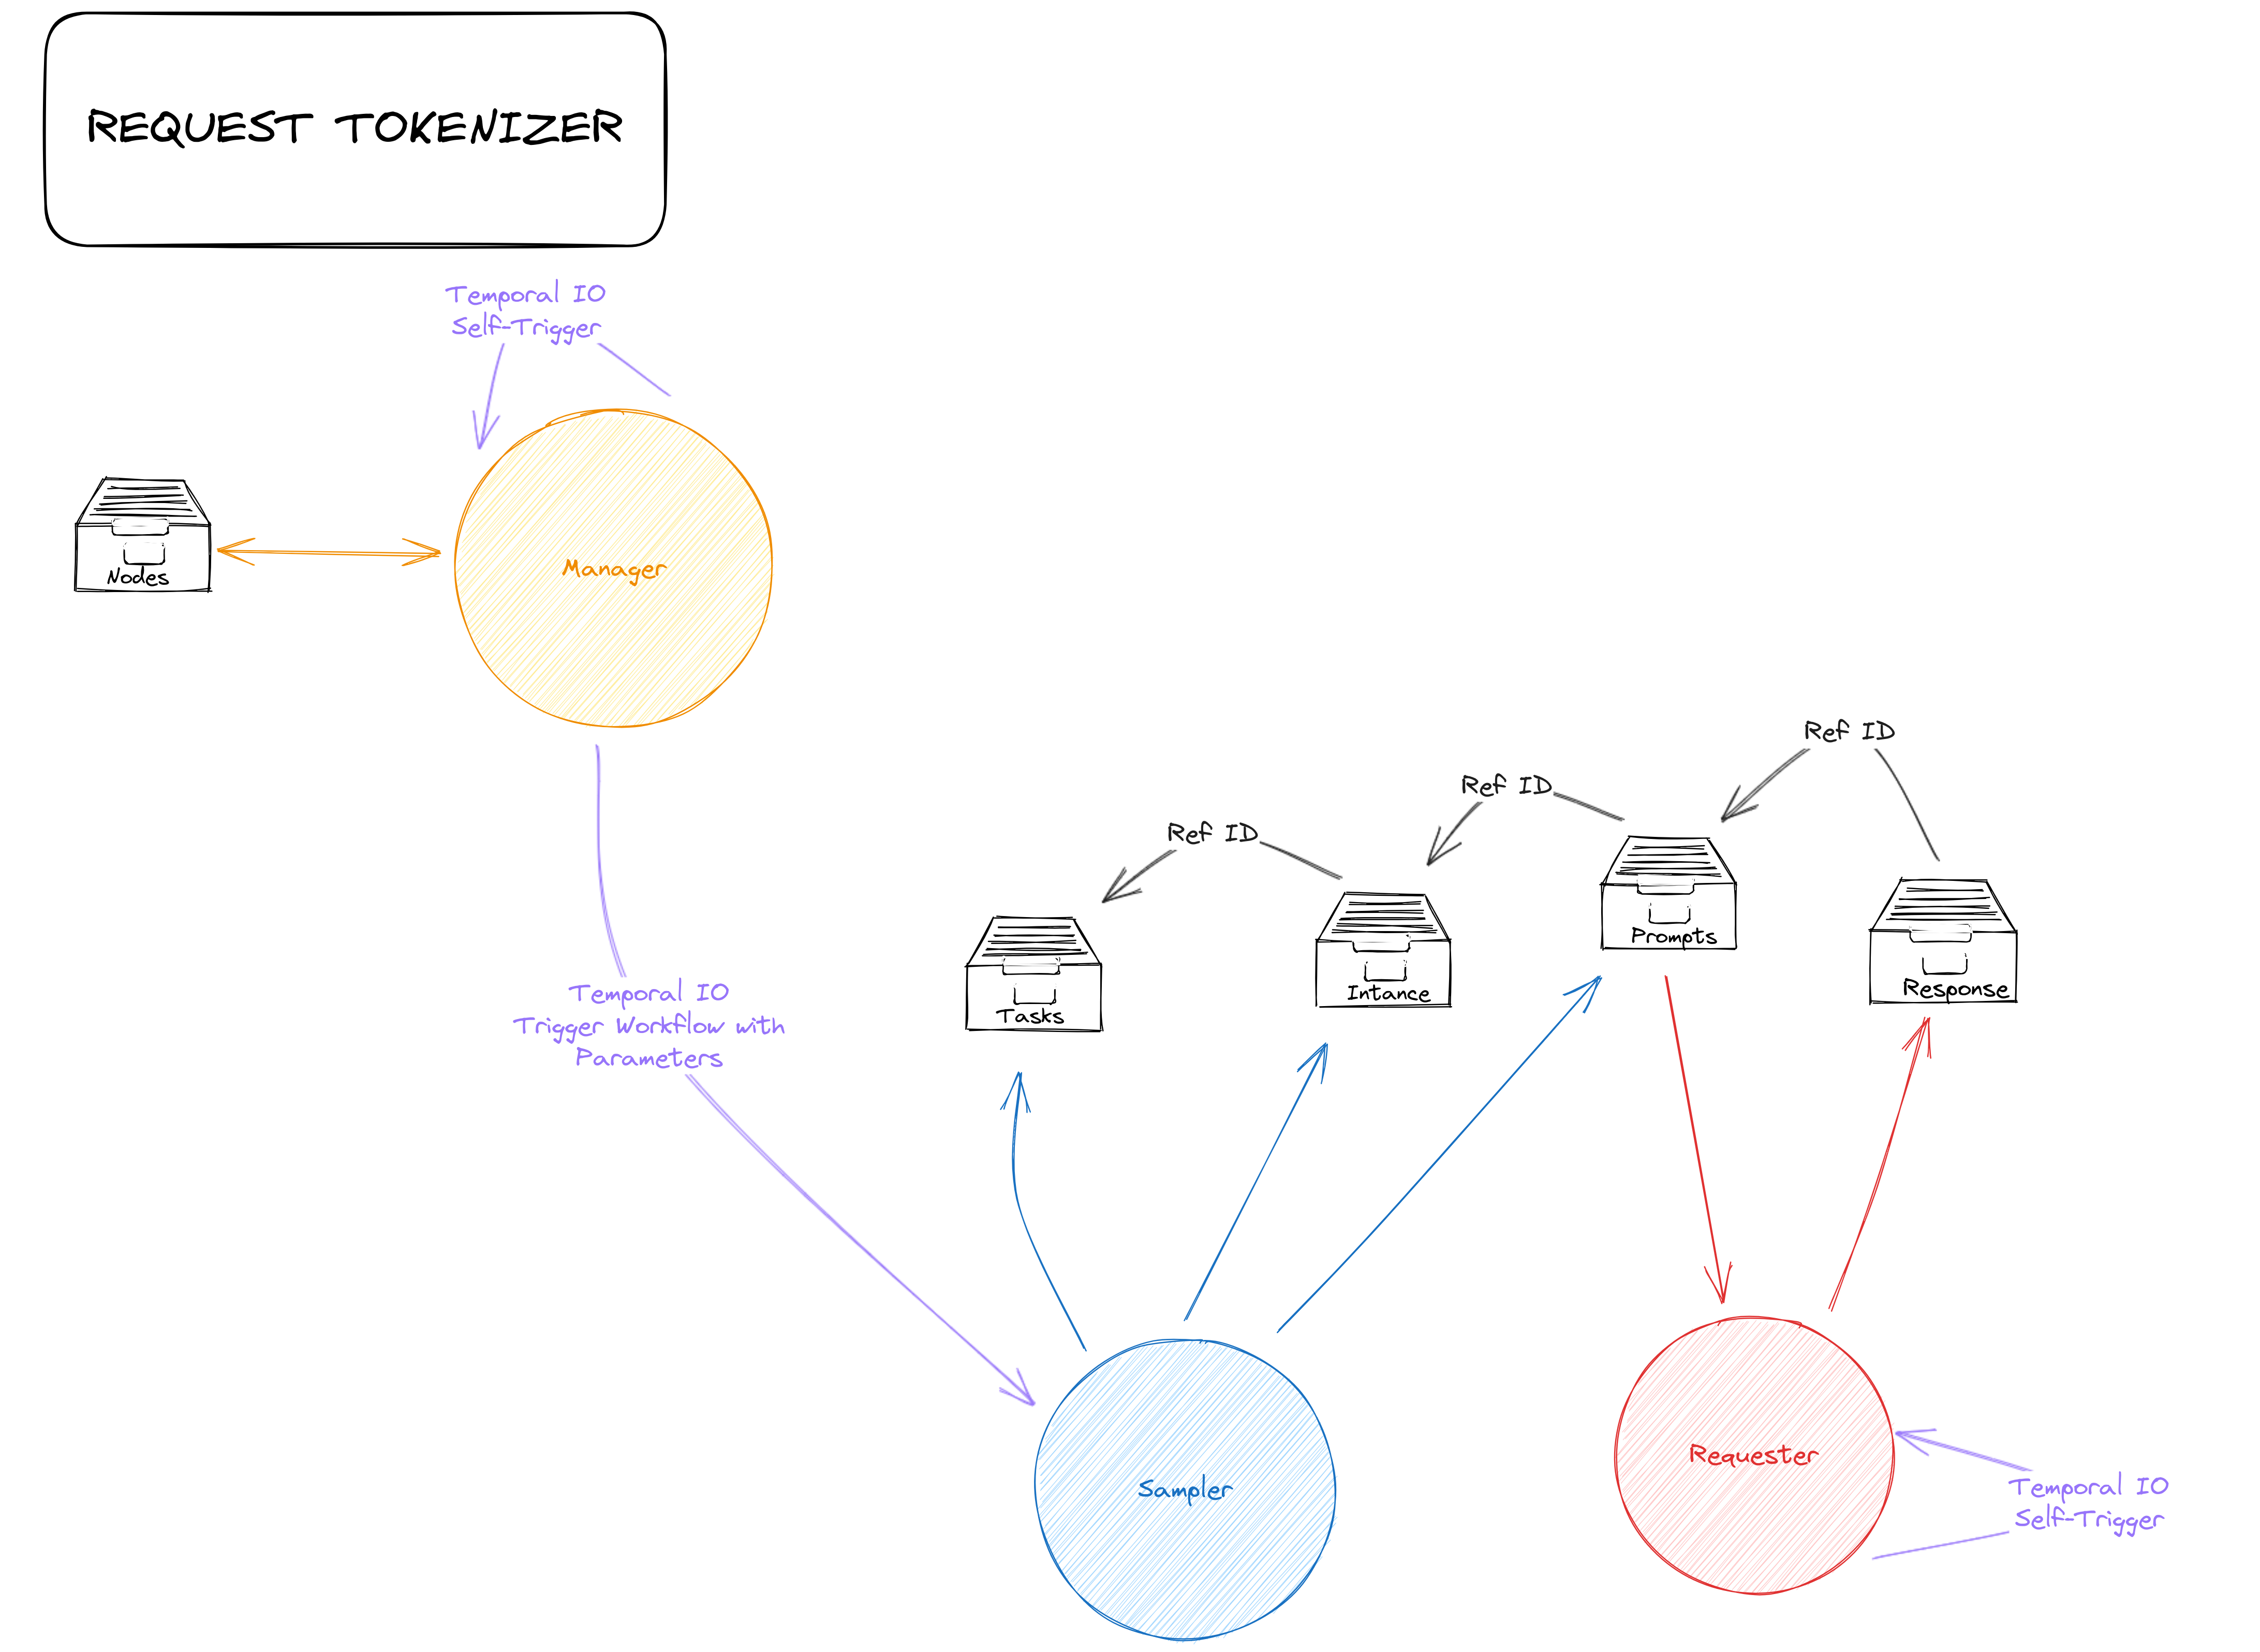
\includegraphics[width=0.8\textwidth]{workflow3}
    \caption{}
    \label{secb:fig:wf3}
\end{figure}

\begin{figure}[H]
    \centering        
    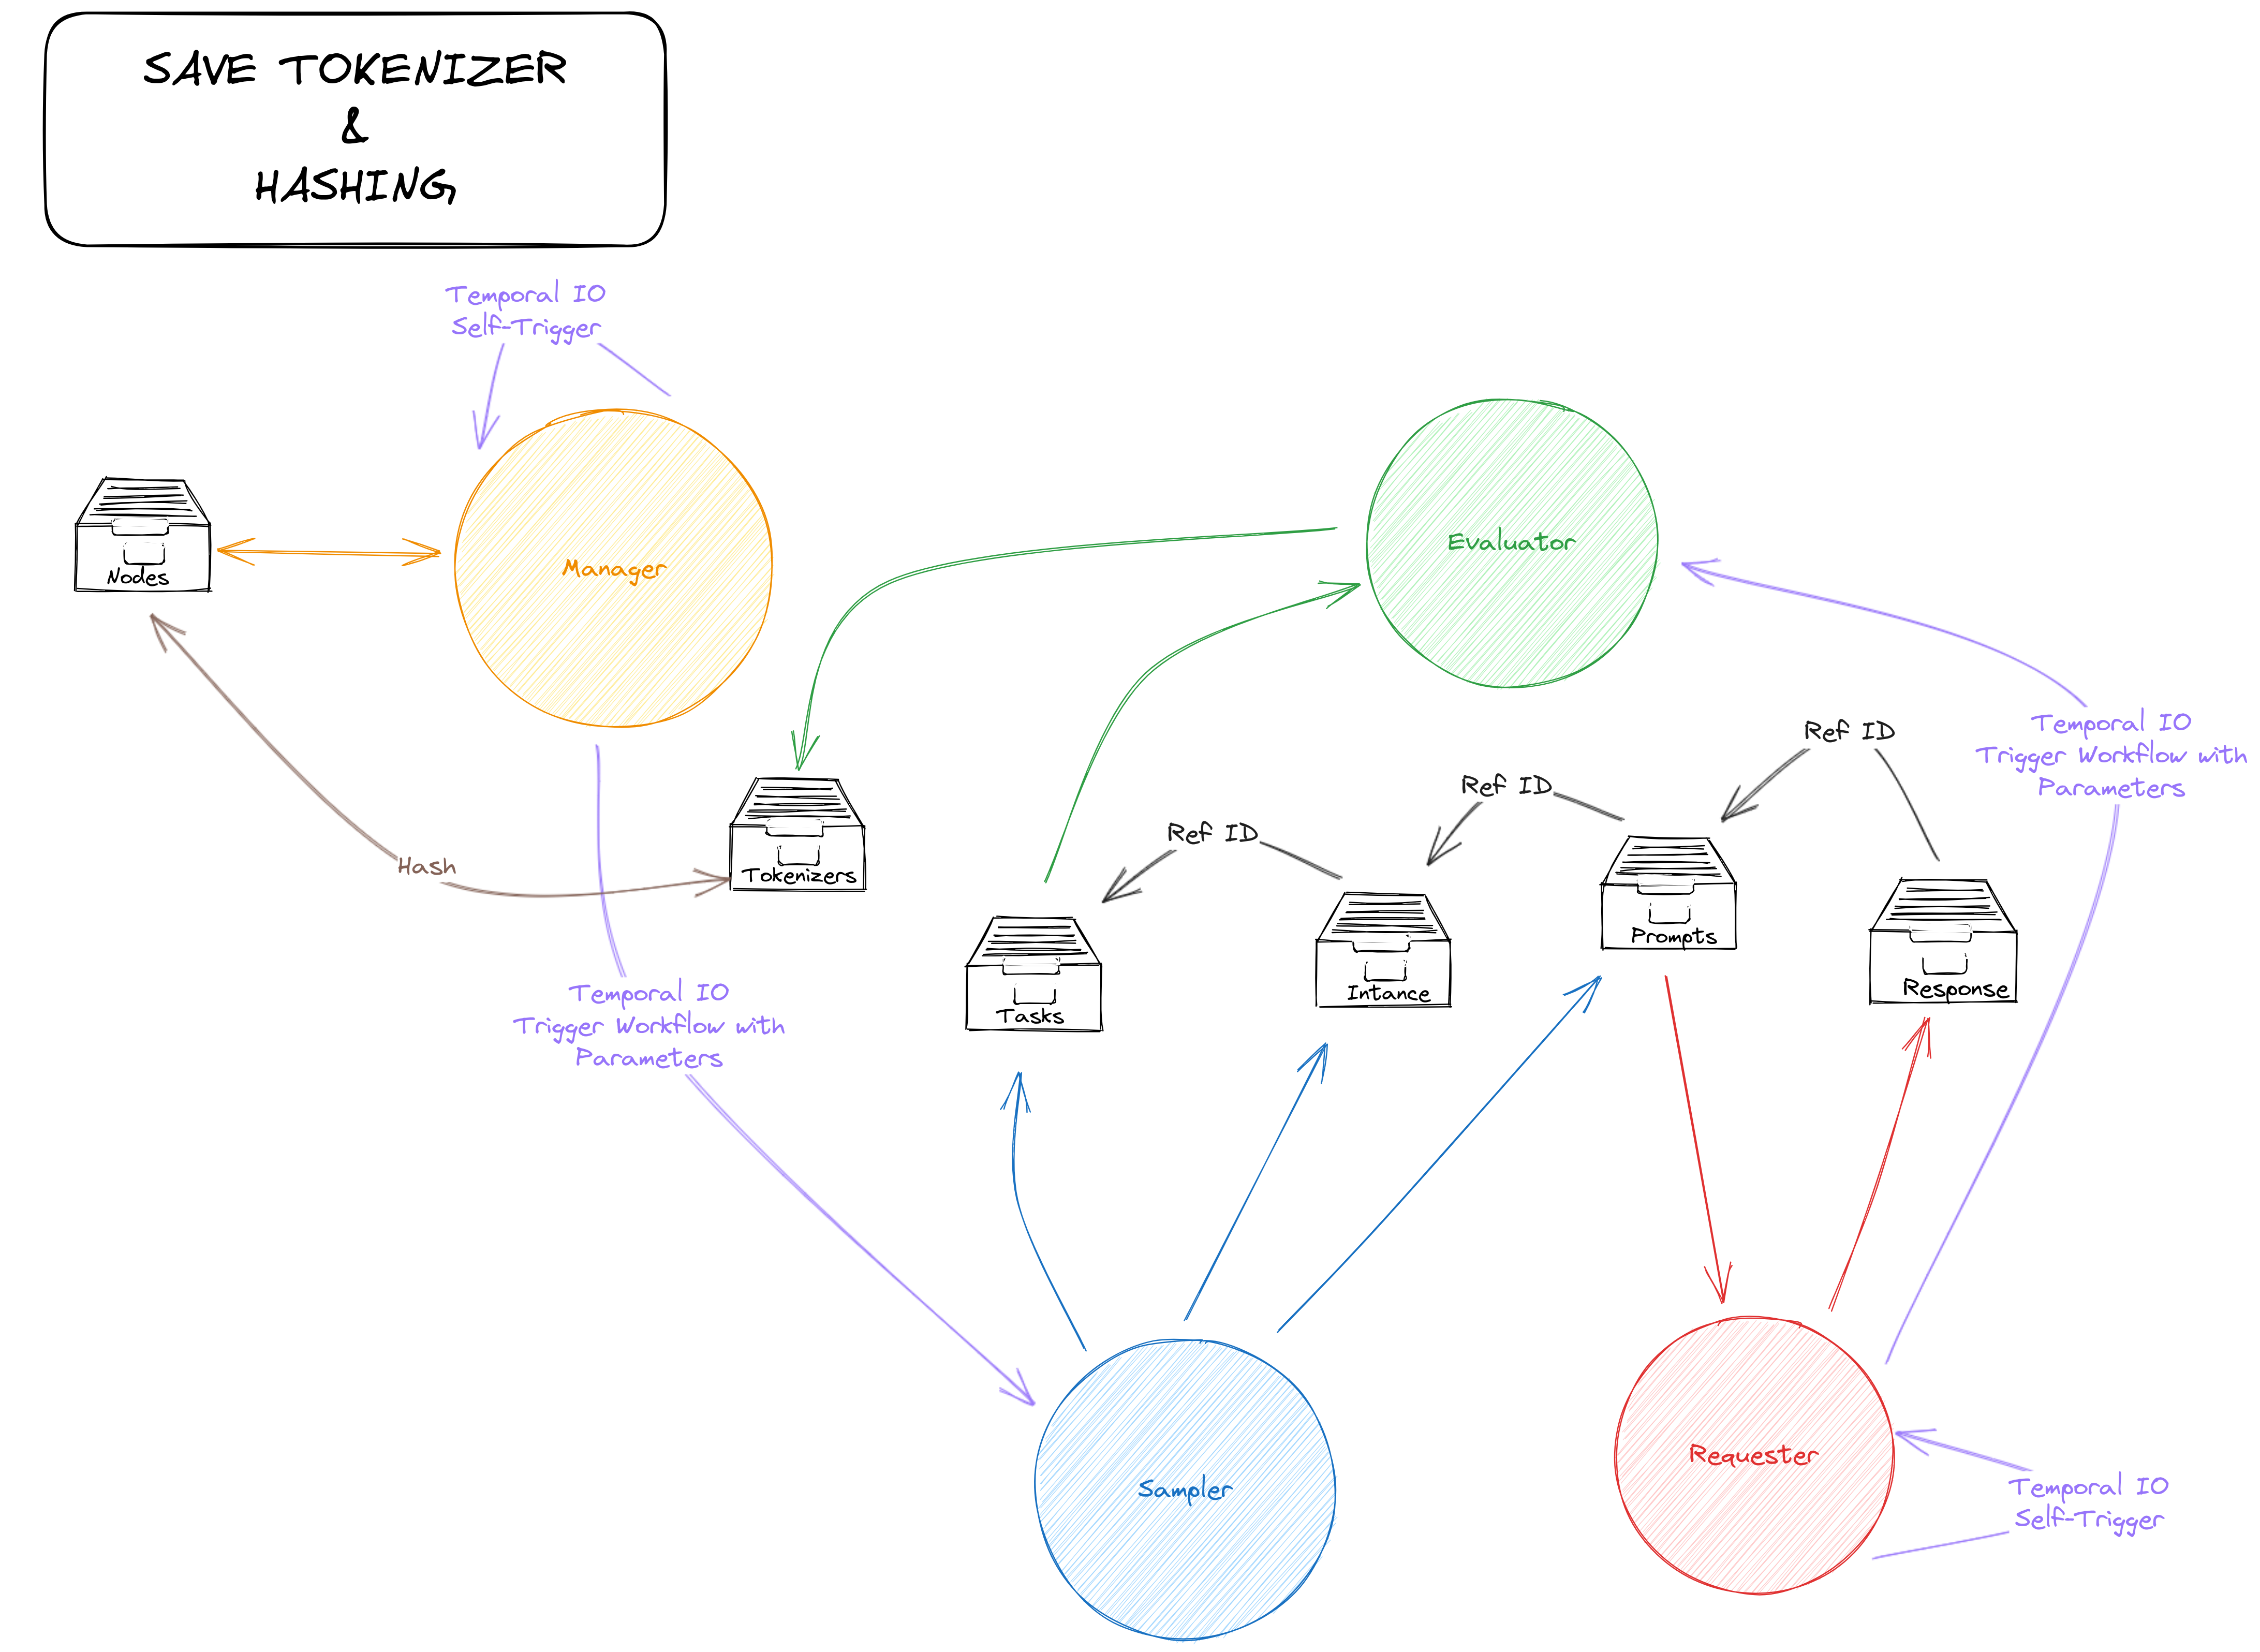
\includegraphics[width=0.8\textwidth]{workflow4}
    \caption{}
    \label{secb:fig:wf4}
\end{figure}

\begin{figure}[H]
    \centering
    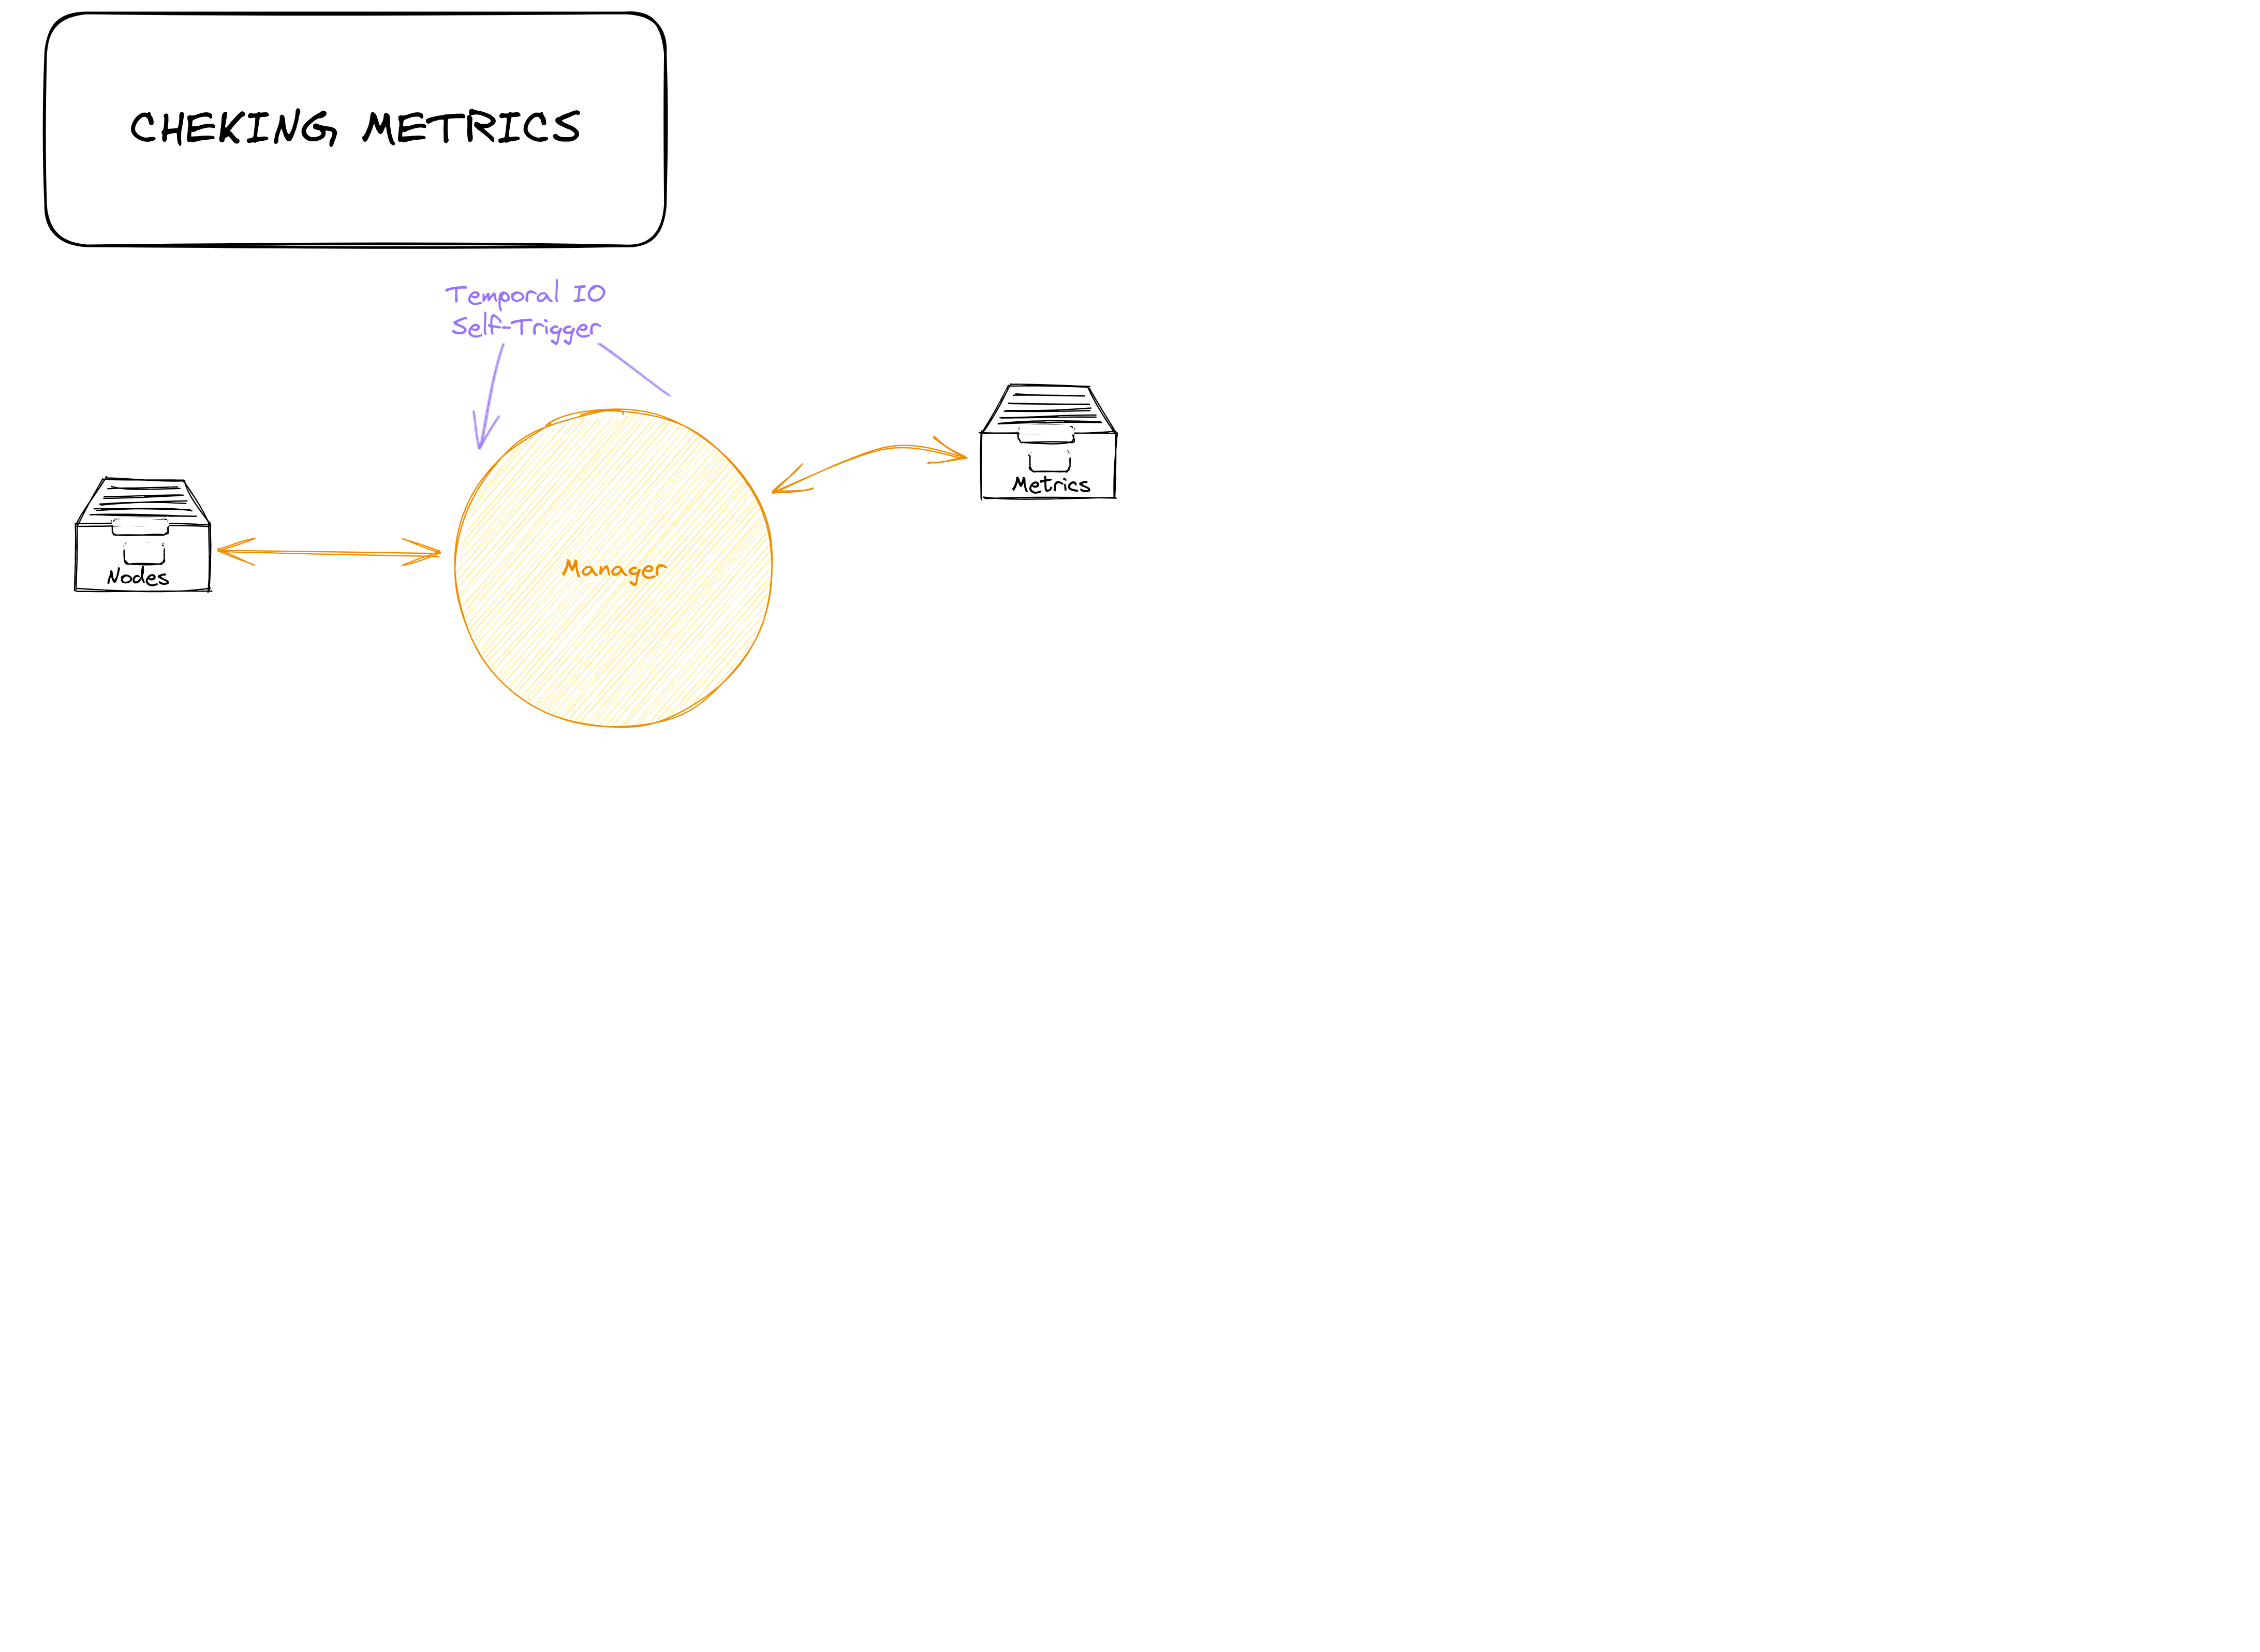
\includegraphics[width=0.8\textwidth]{workflow5}
    \caption{}
    \label{secb:fig:wf5}
\end{figure}

\begin{figure}[H]
    \centering
    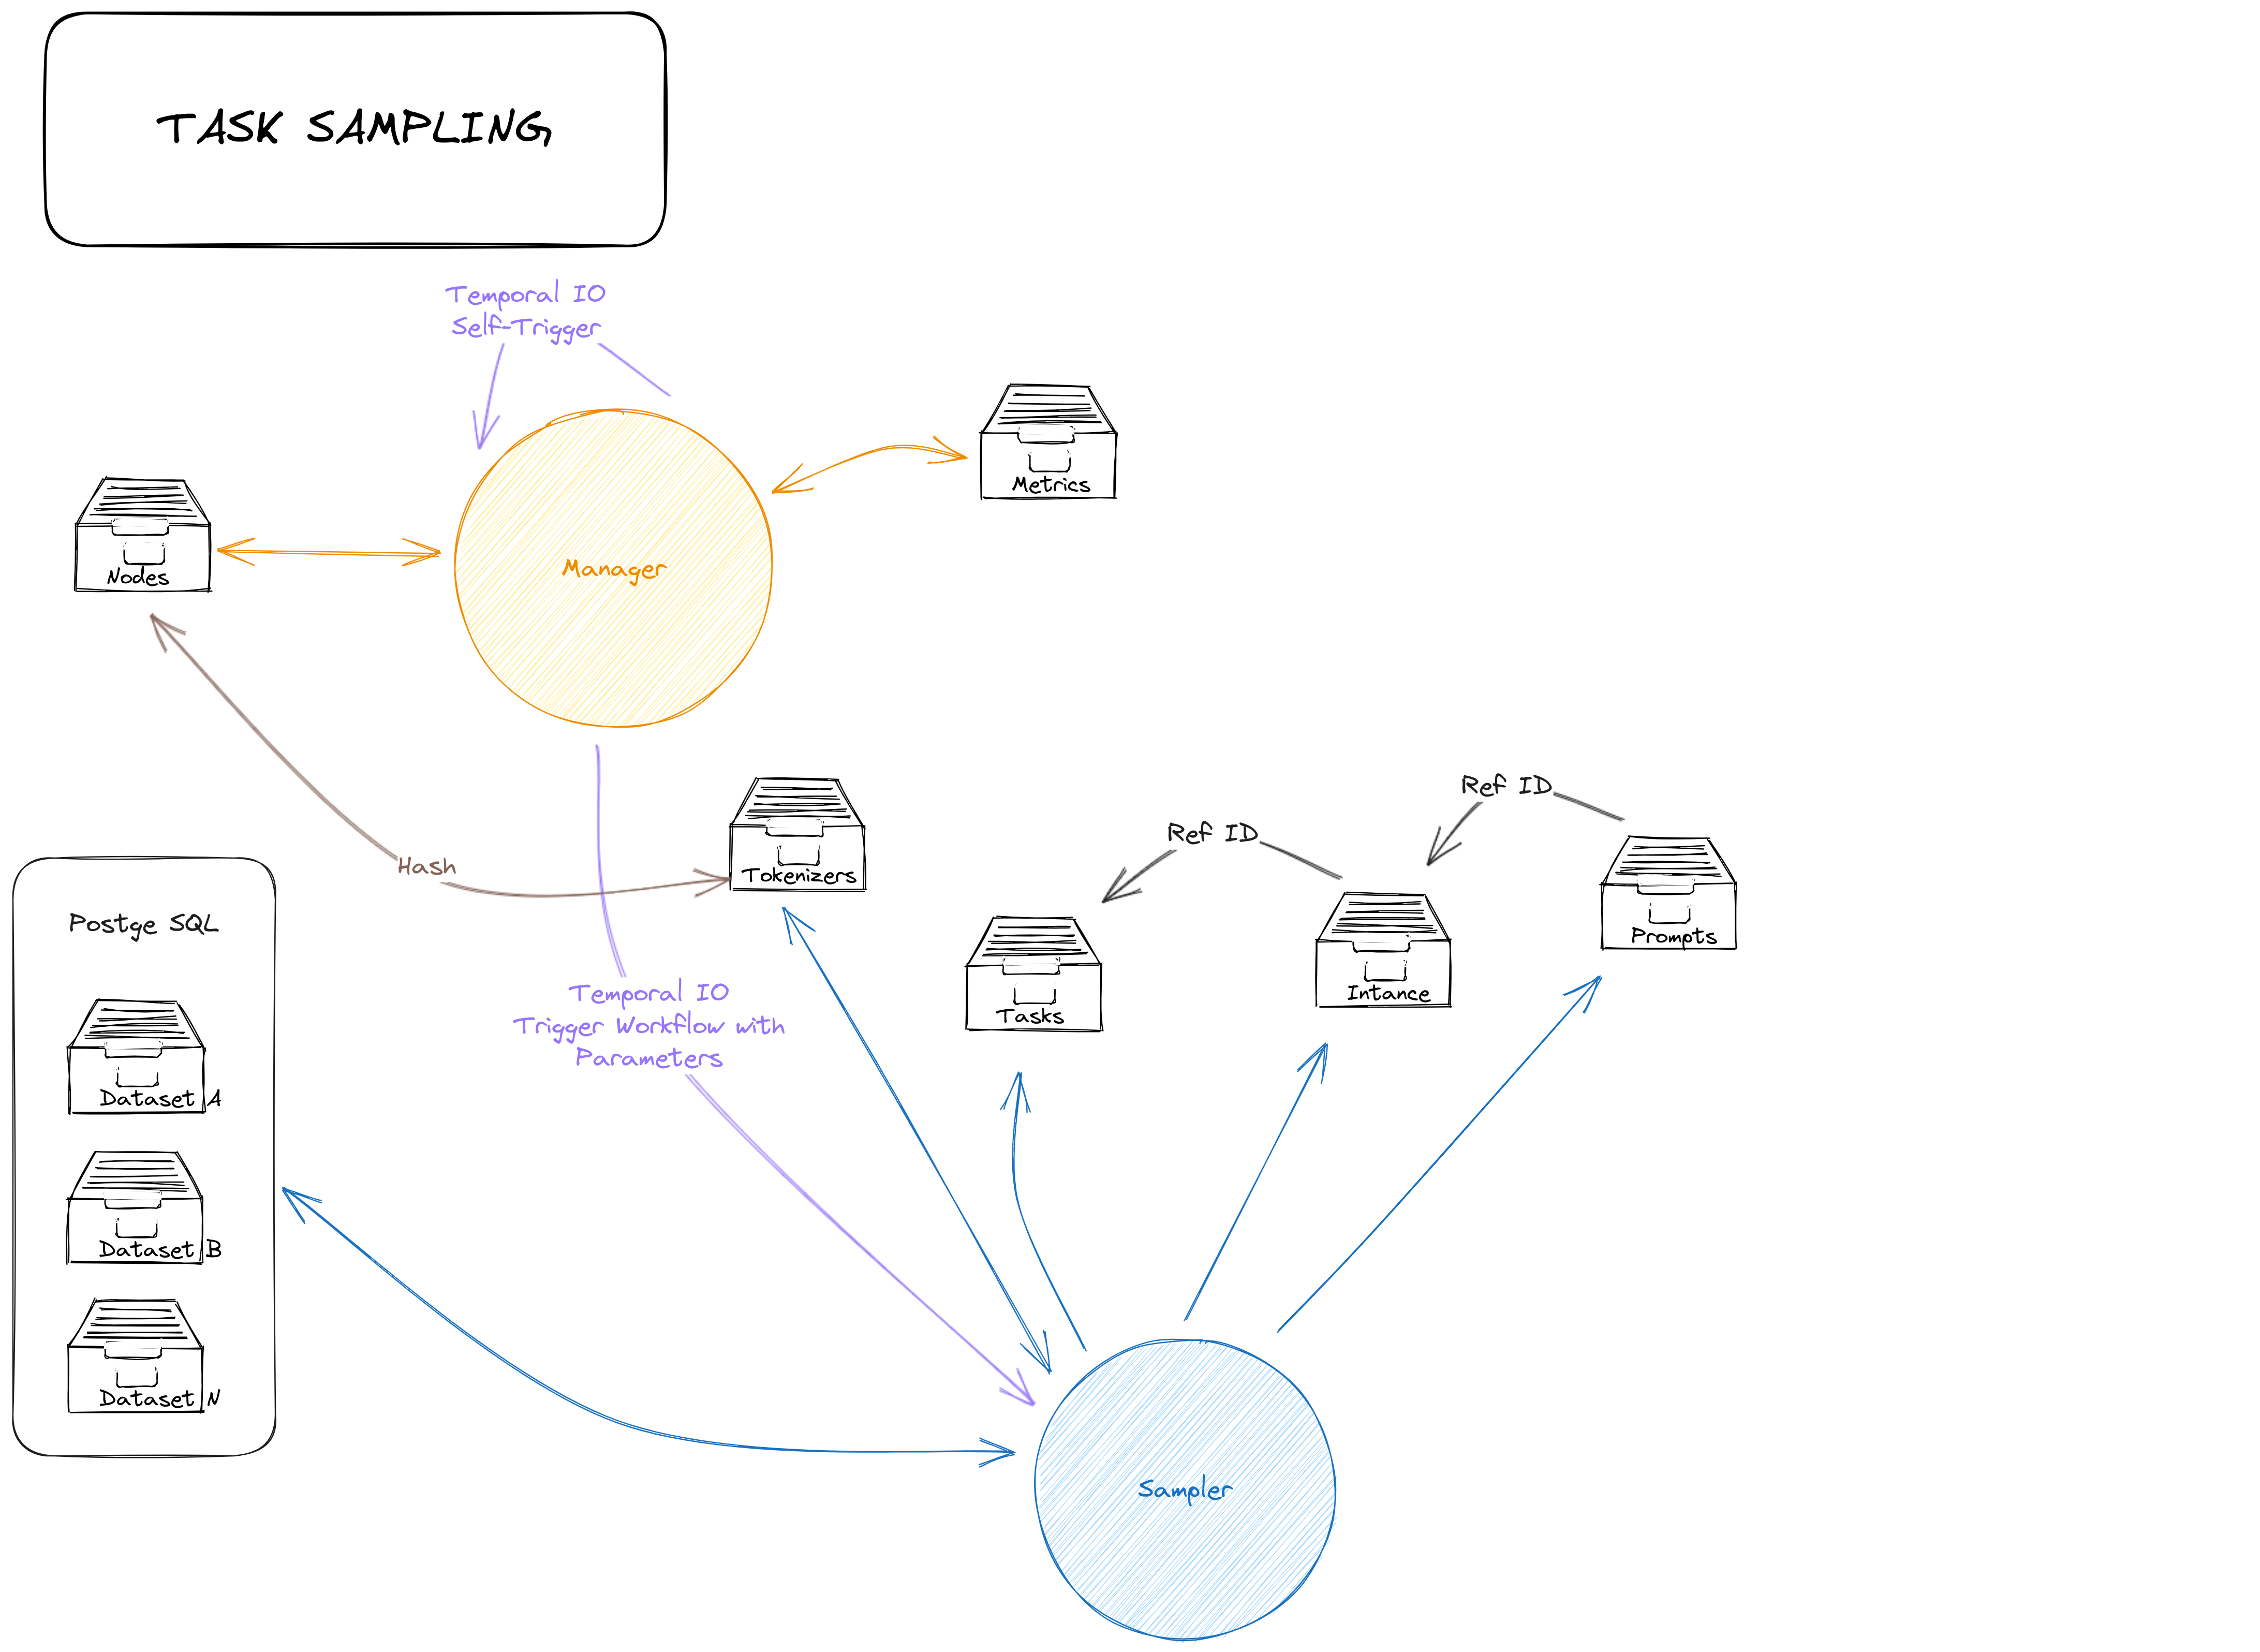
\includegraphics[width=0.8\textwidth]{workflow6}
    \caption{}
    \label{secb:fig:wf6}
\end{figure}

\begin{figure}[H]
    \centering
    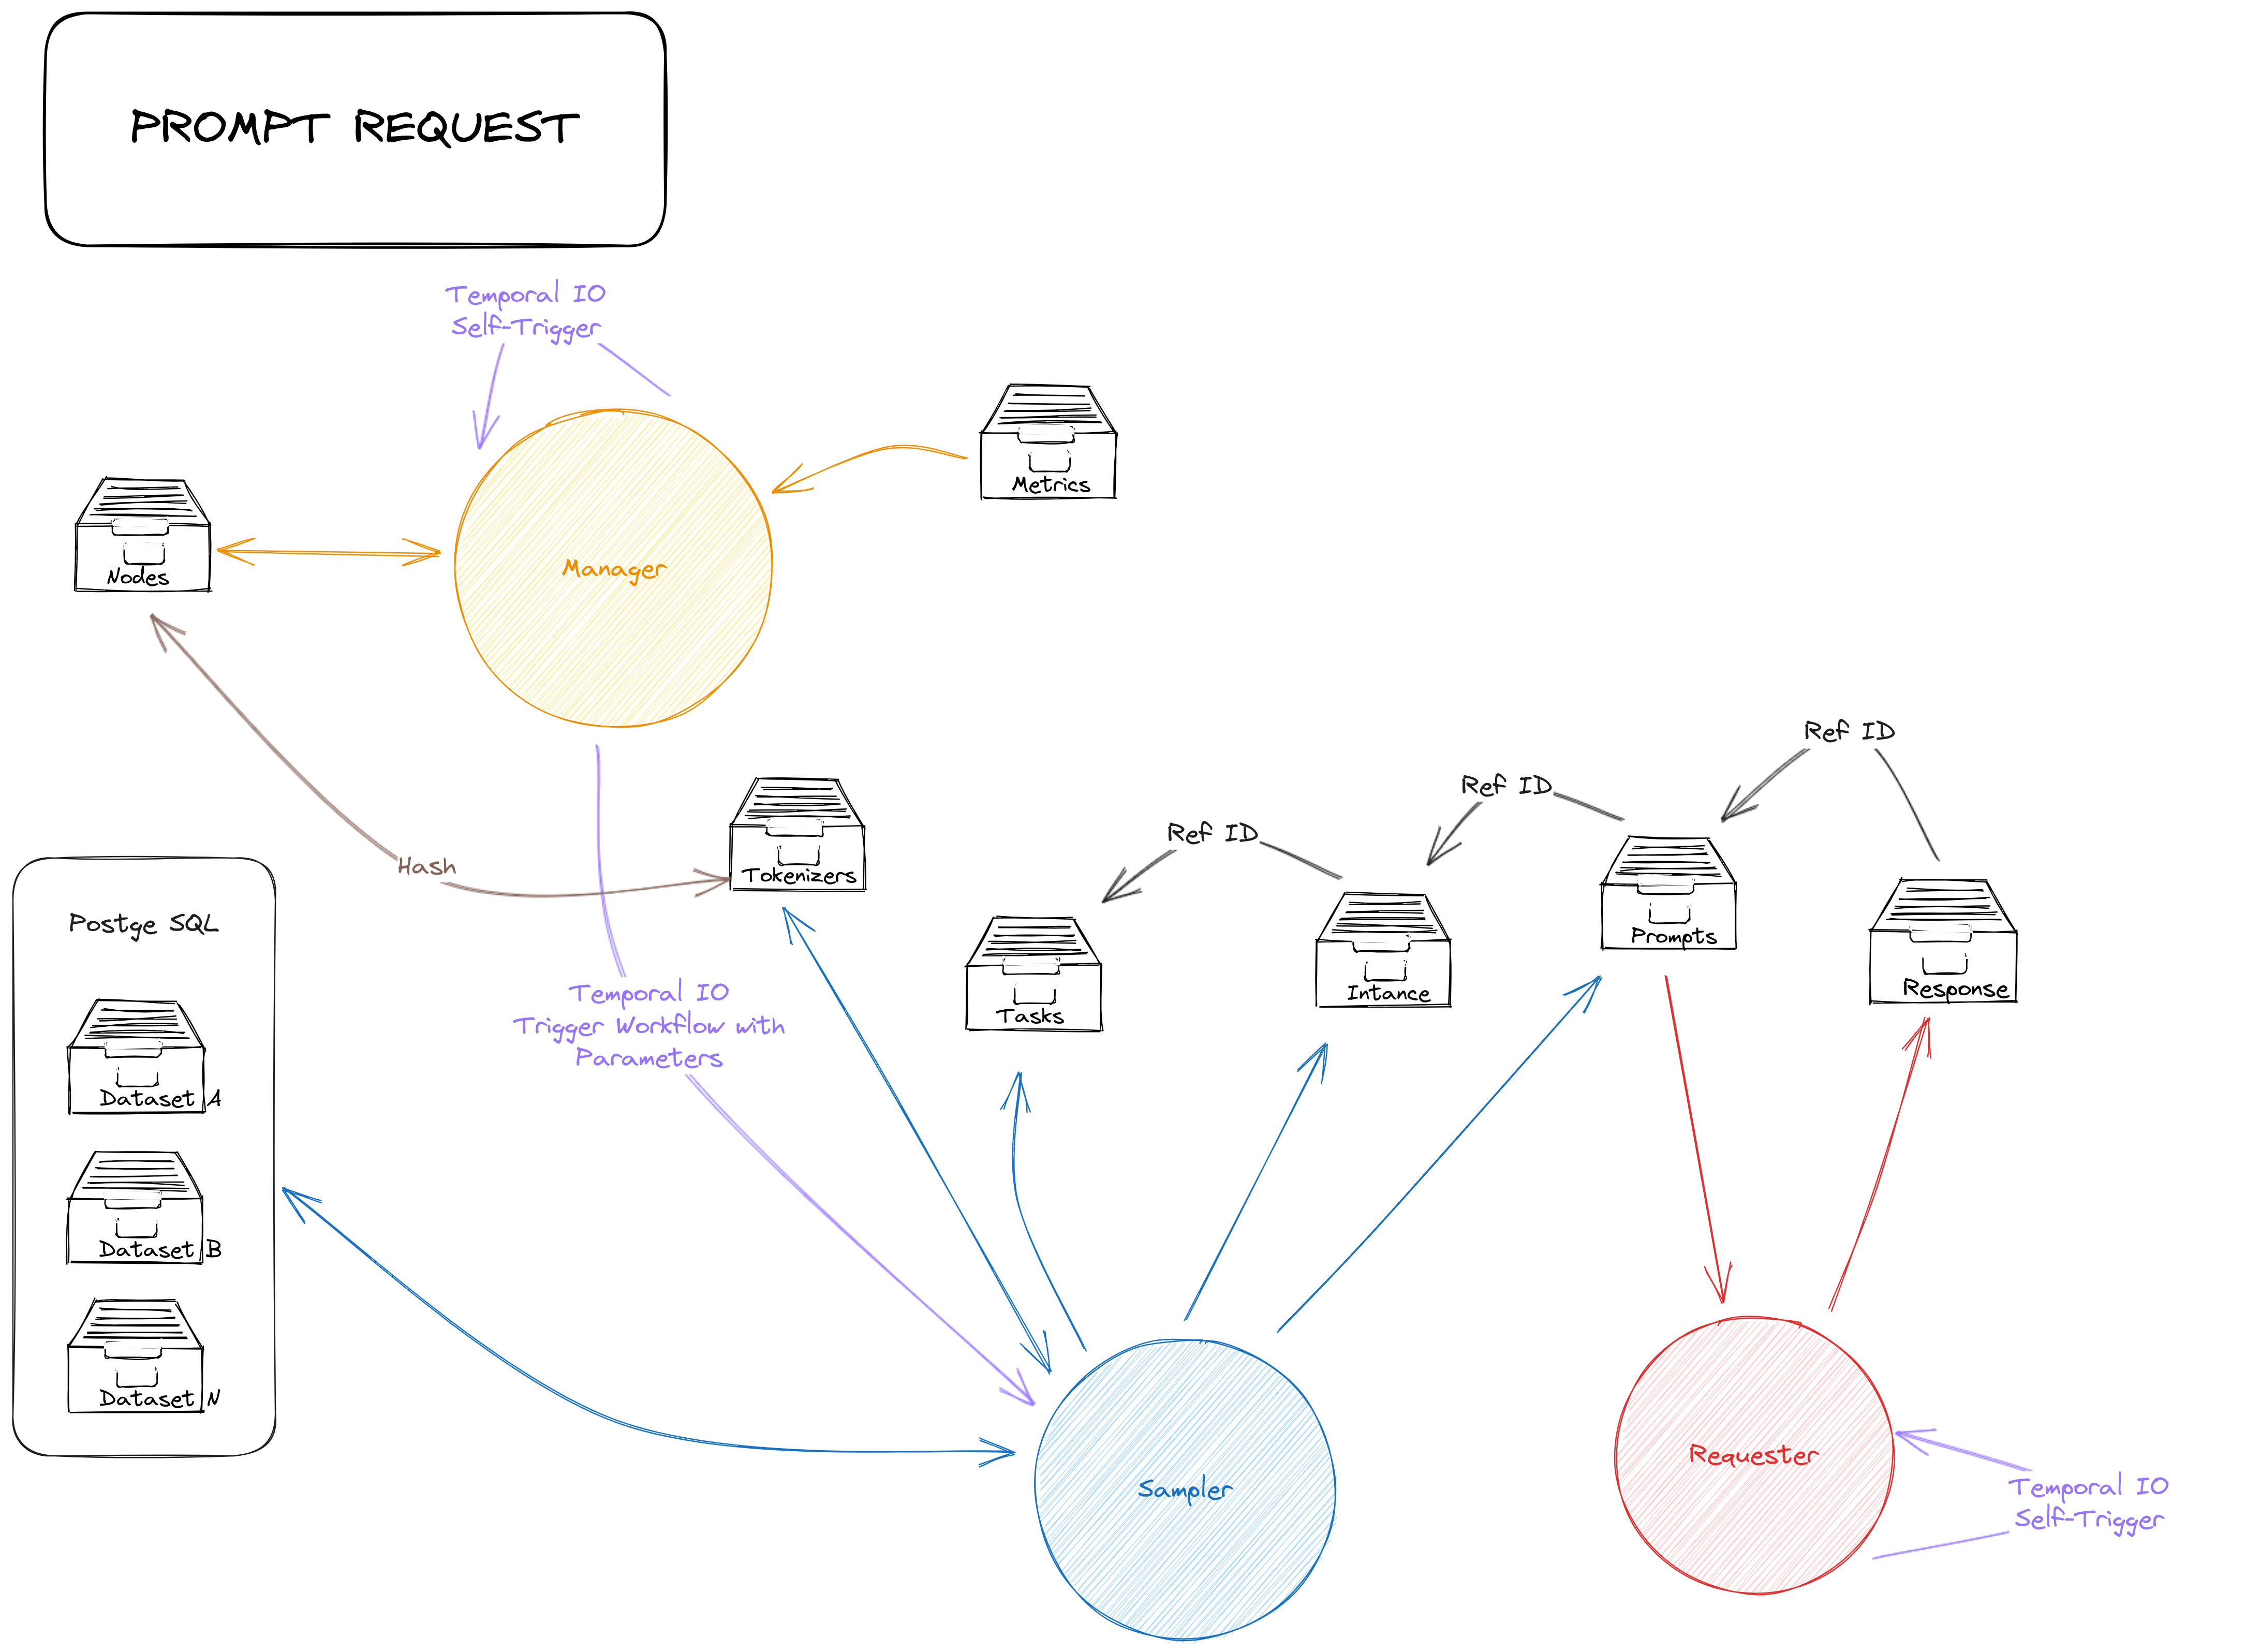
\includegraphics[width=0.8\textwidth]{workflow7}
    \caption{}
    \label{secb:fig:wf7}
\end{figure}

\begin{figure}[H]
    \centering
    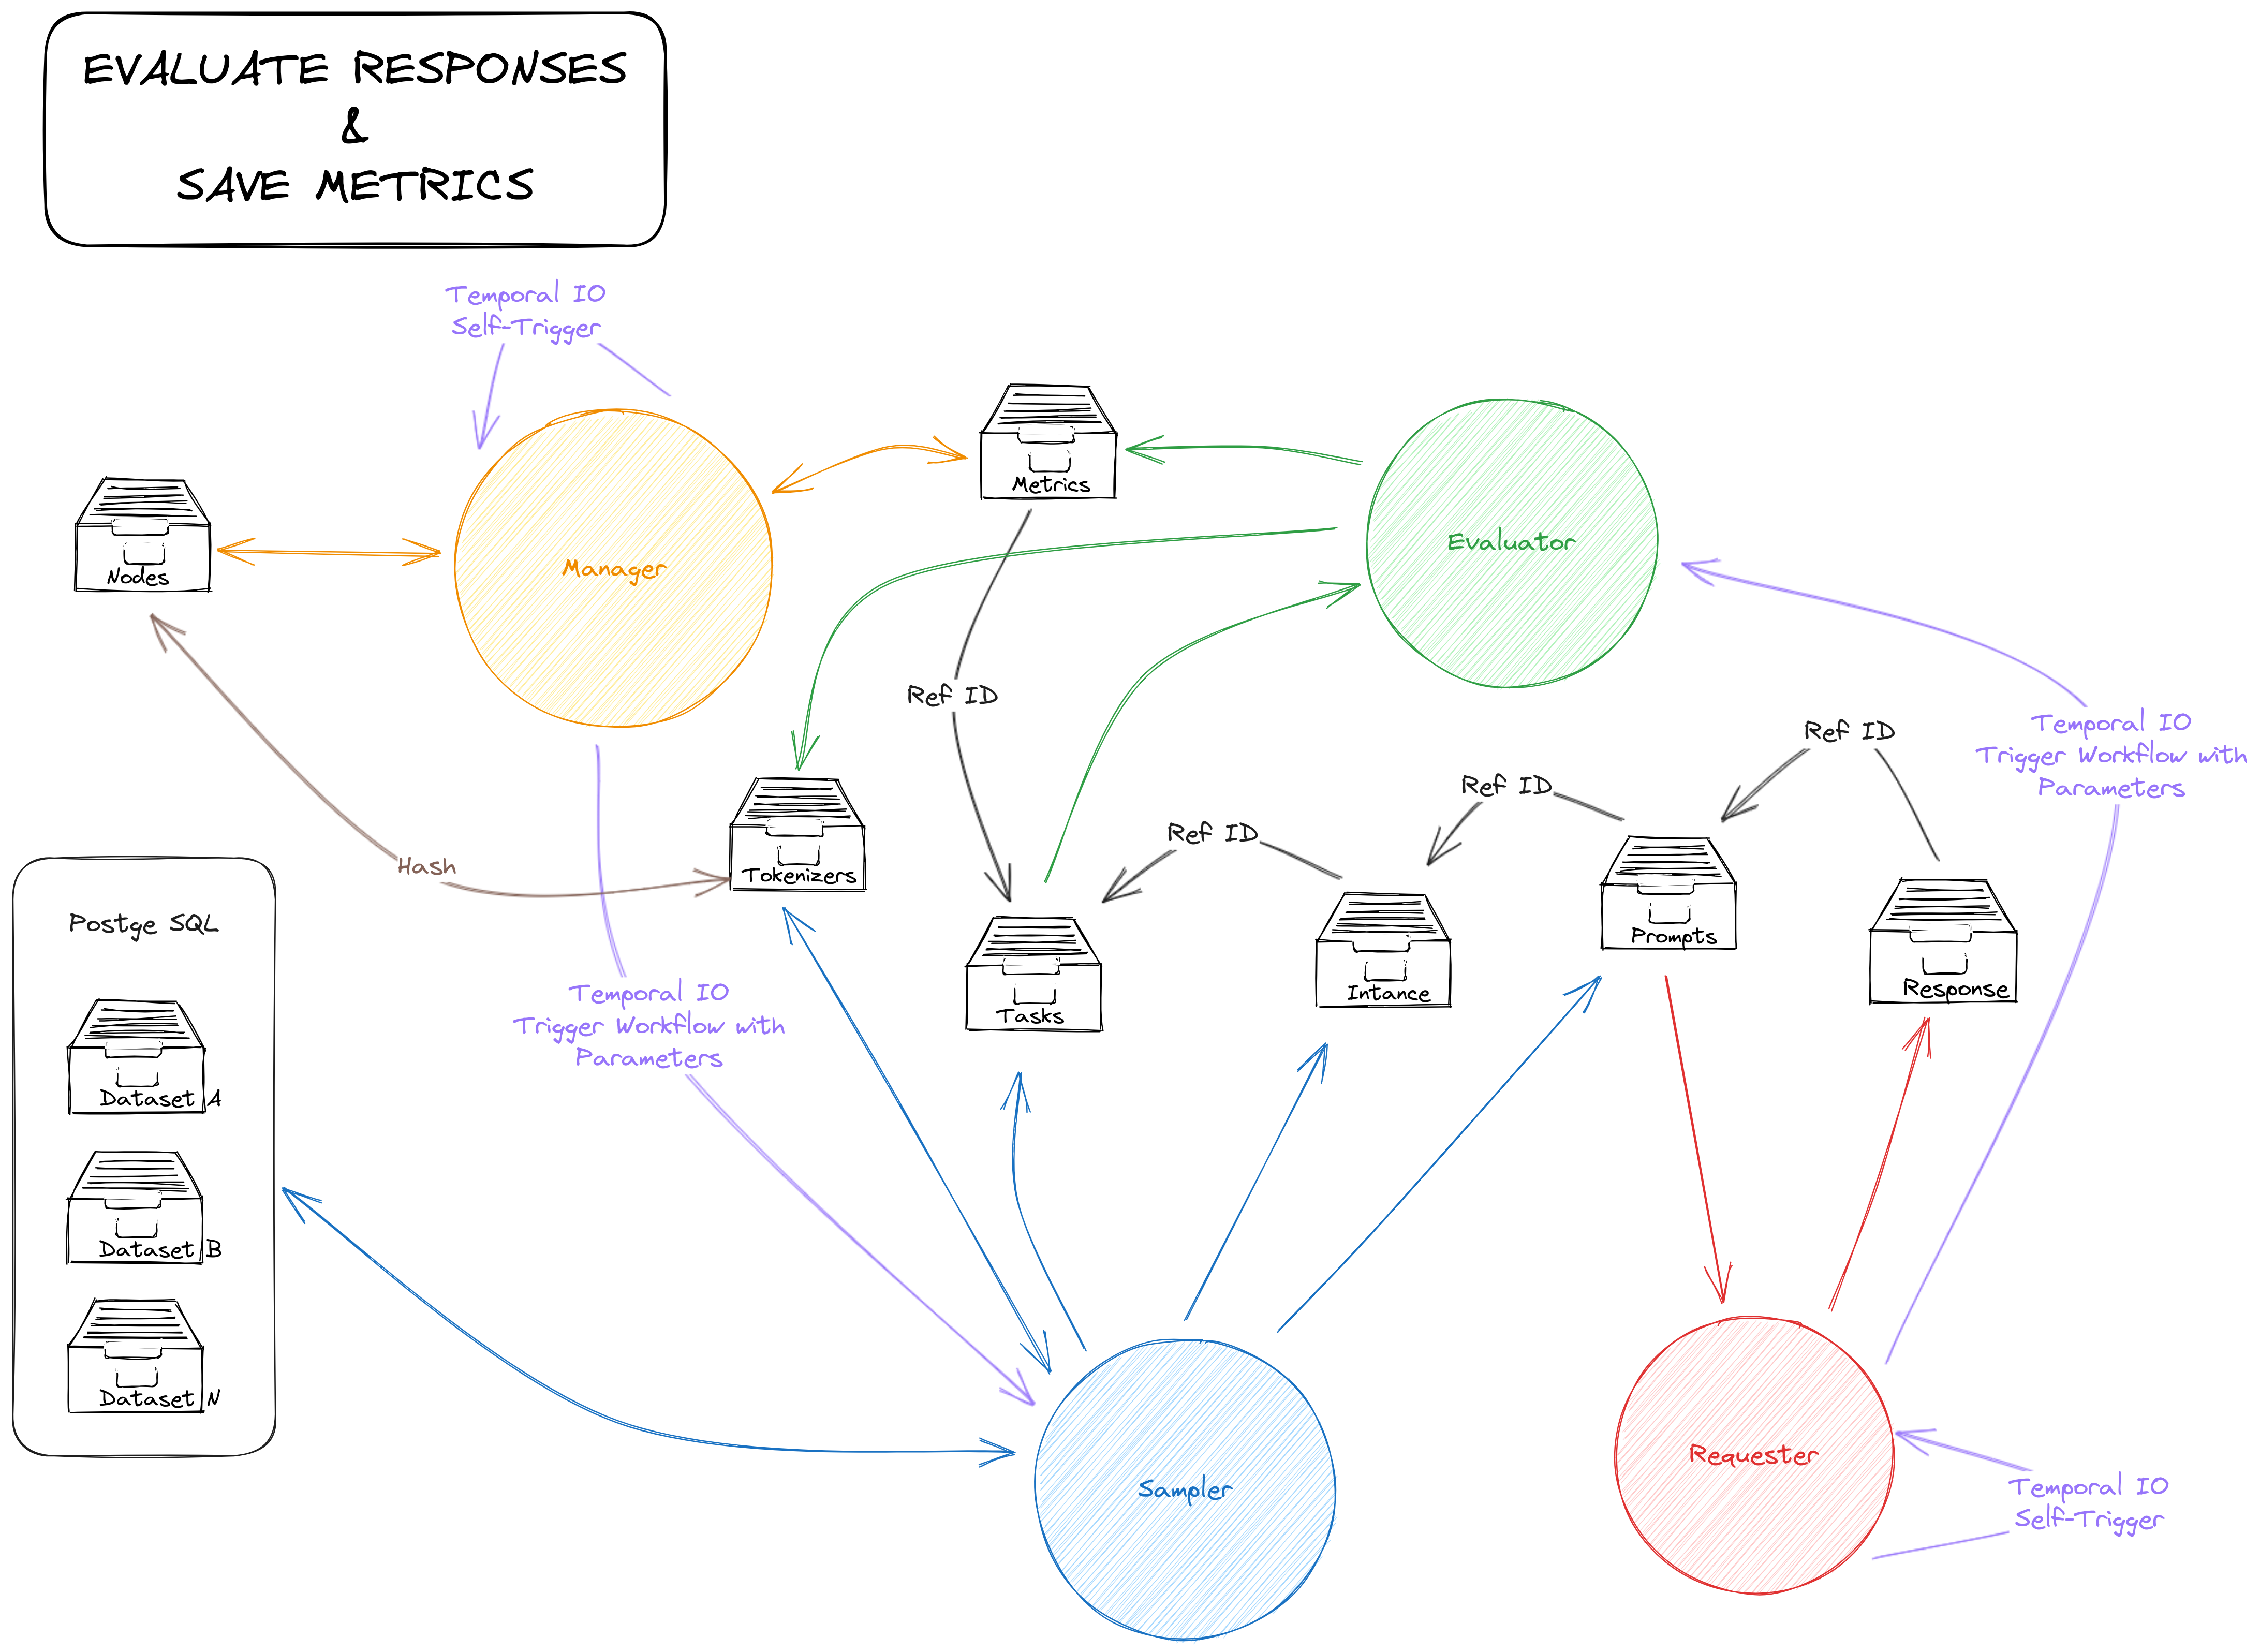
\includegraphics[width=0.8\textwidth]{workflow8}
    \caption{}
    \label{secb:fig:wf8}
\end{figure}

\begin{figure}[htb!]
    \centering
    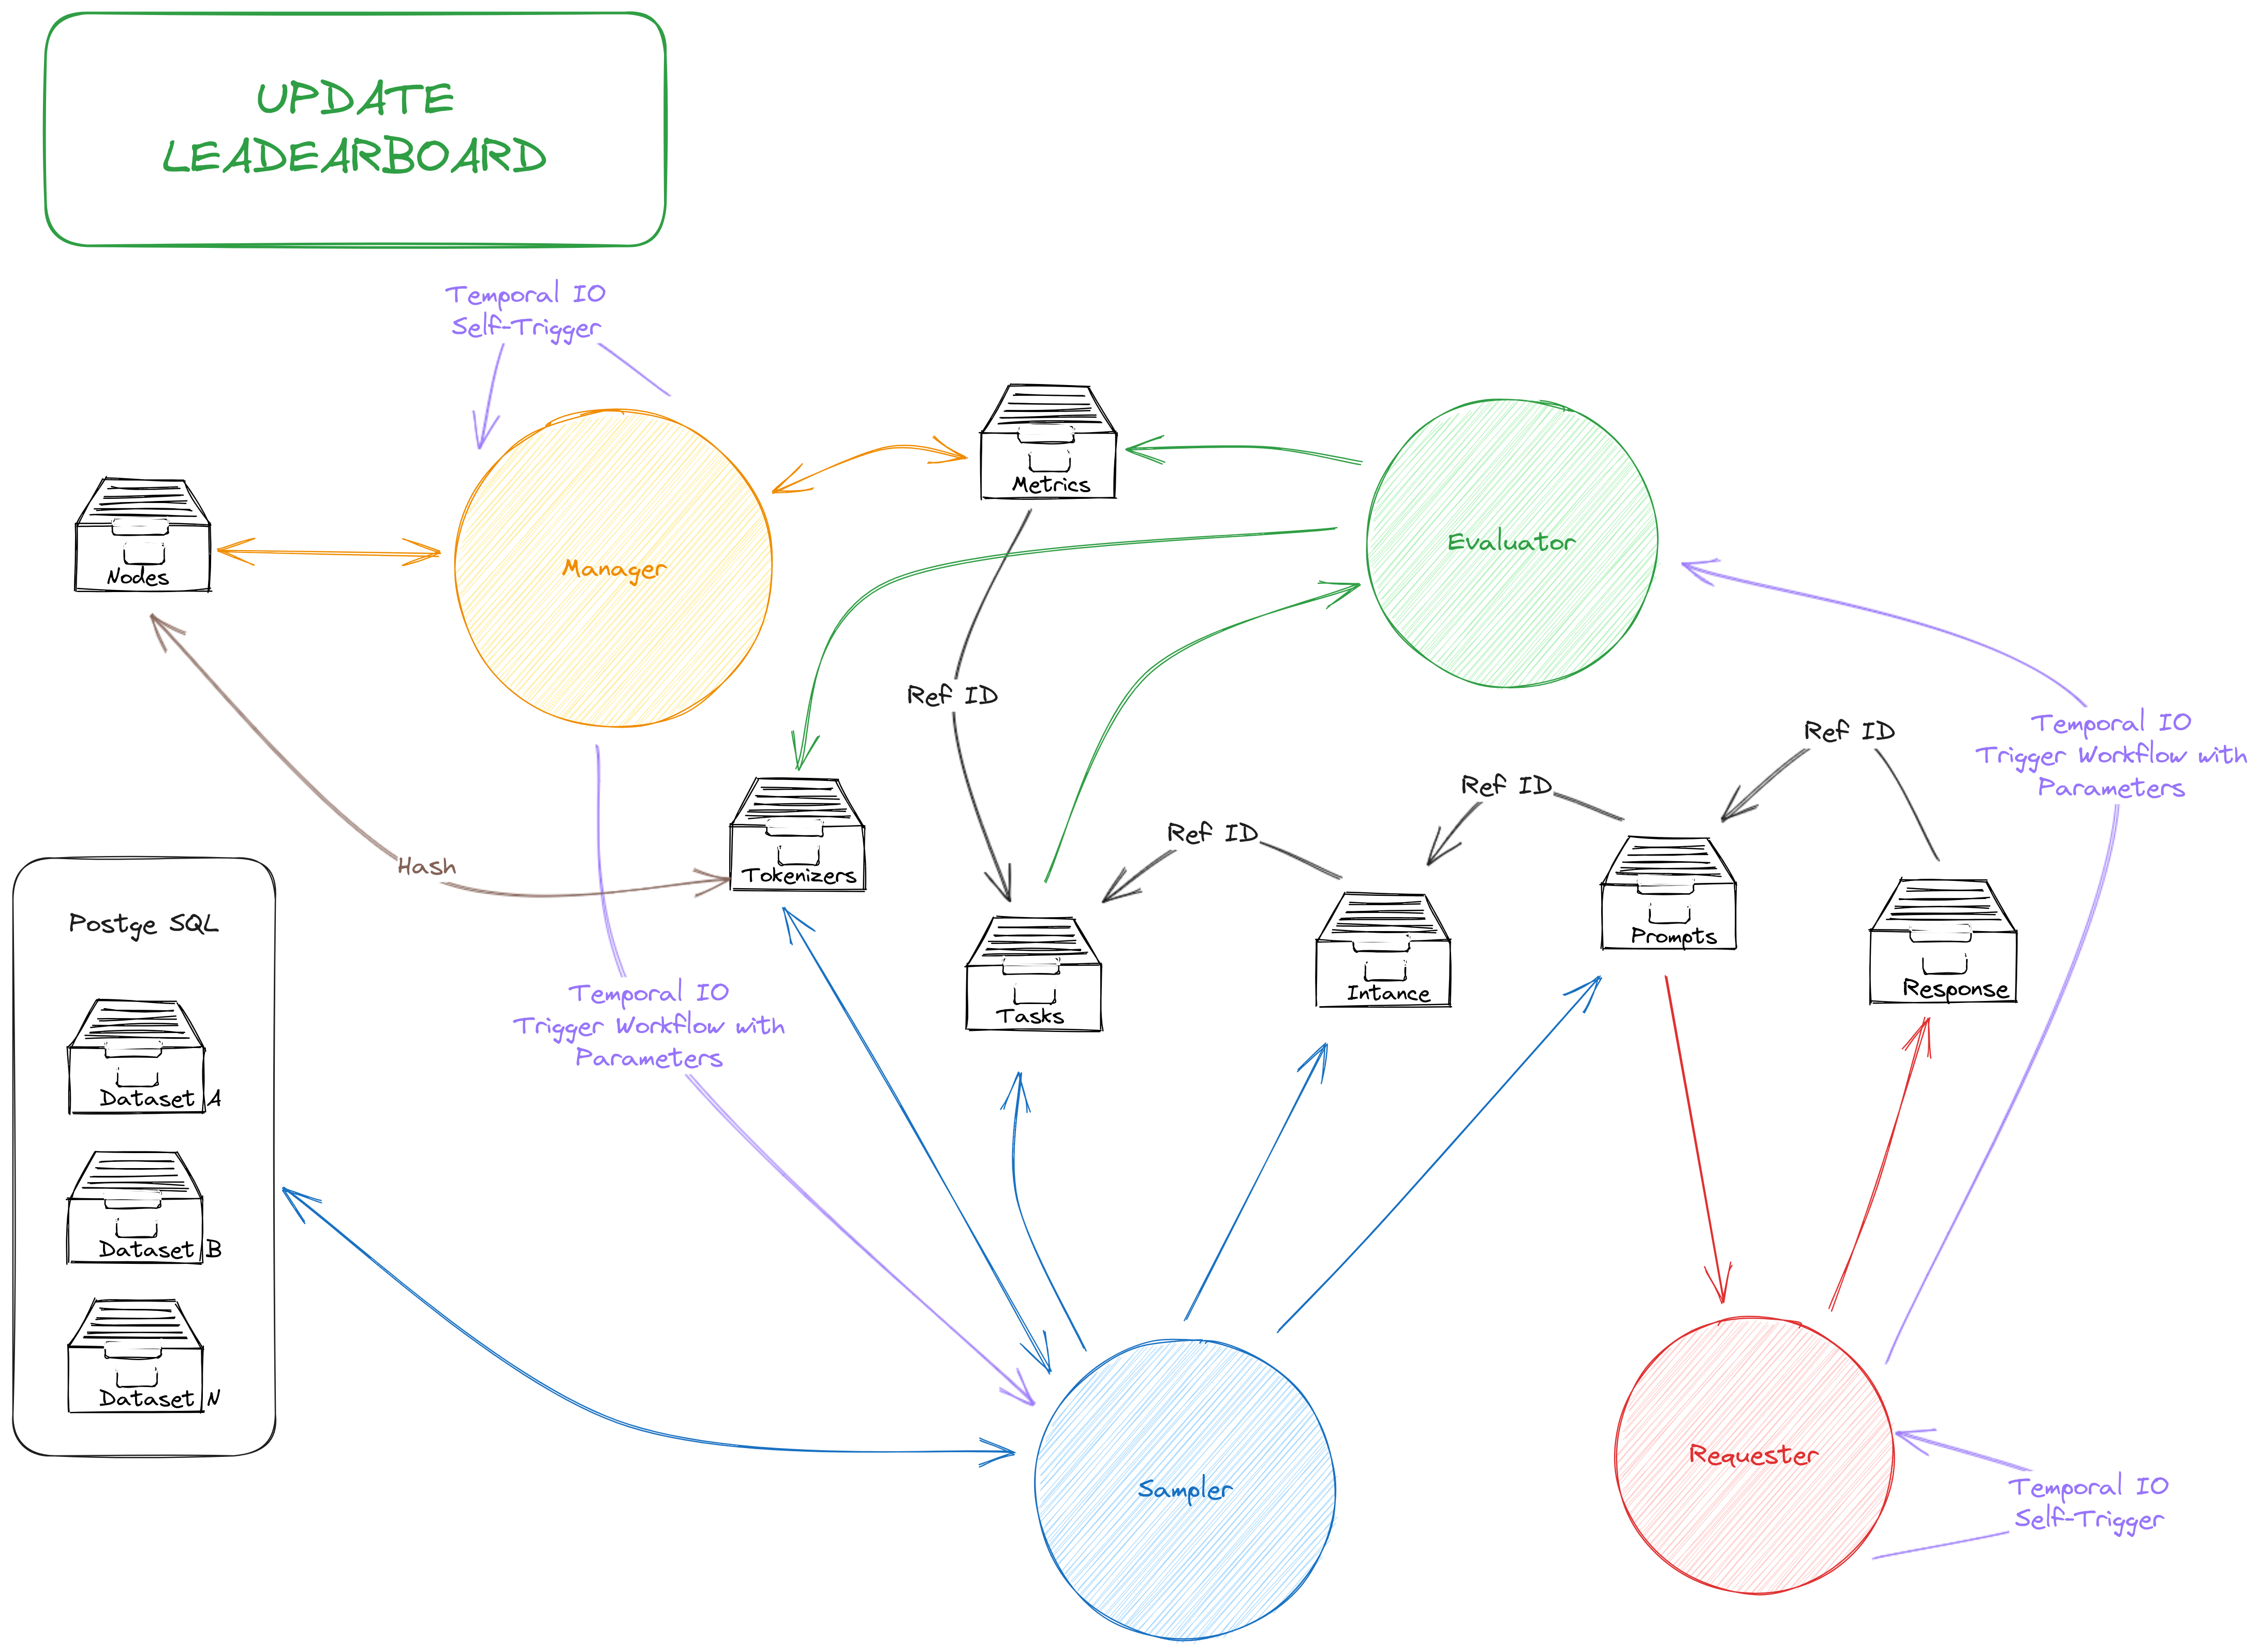
\includegraphics[width=0.8\textwidth]{workflow9}
    \caption{Update metrics.}
    \label{secb:fig:wf9}
\end{figure}

Manager detect nodes staked, checking signatures for example tokenizers. If the node has not a signature/tokenizer associated, it will be requested. 
If signatures are ok, then it will check if the model requires new samples to update any task/metrics. 
when is required (low threshold of the samples required), trigger sampler. 
During the creation of the samples, the tokenizer is called, and prepare the prompt. 
The requester check if there is any prompt not done, and send to trhougth the network. 
Once each sample from a task is done, the requester marks the task as done. 
Due to Evaluator is scanning for tasks done, it will start the evaluation of each sample, then saving the results in the database. 

\subsection{Workflows}

Consider a scenario where nodes $N$ are staked in service $S$ ... \textcolor{red}{COMPLET}

Then, the main steps are the following:

\paragraph{Cheking signatures:}
The Manager will check if $N$ in $S$ has a signature $\sigma$ associated in the nodes collection. 
If not, it will request it. 
In the particular case of testing \gls{LM}, its signature consists of a hash of its tokenizer $T$, hereafter referenced as $\sigma(T)$. 
In ease of expression, we will refer to the signature of node $N$ in $S$ as $\sigma(T_{N}^{S})$. 
Figure \ref{secb:fig:wf1} shows the workflow until this step.


\paragraph{Sample tokenizer:}
To produce the signature, the Manager triggers the Sampler module to save a prompt for the Requester pointing to the endpoint of $N_s$ in the \textit{prompts} collection. |textcolor{red}{COMPLET WITHMORE DEITAL ABOUNT SIDECARD?}
Figure \ref{secb:fig:wf2} shows the workflow until this step.


\paragraph{Request tokenizer:}
When $N$ is serving in a session, the app \textcolor{red}{(explain how the app will work?)} will send a request with the prompt, and the node will respond with the a json tokenizer $T$.  glorify the occasional fulfillment of that function, to treasure old and foreign thoughts, to recall
with incredulous amazement what the doctor universalis thought, is to confess our languor or ourection \textit{tokenizers}, noting that if many nodes have the same tokenizer, it will be saved only. 
Figure \ref{secb:fig:wf4} shows the workflow until this step.


\paragraph{Checking metrics:}
Once a node has its signature, the Manager will check if any sample related to a metric of a task needs to be updated, either because the configured time has expired, or it does not yet have a sufficient number of samples to produce reliable metrics. 
If required, the Manager will trigger the Sampler, requiring from the Sampler a quantity $q$ of samples for the task. 
Figure \ref{secb:fig:wf5} shows the workflow until this step.


\paragraph{Task sapling:}
When the Sampler receives the request from the Manager, it will load the dataset corresponding to the task but avoiding to load samples previously requested from the evaluation dataset. 
The Sampler randomly selects $q$ docs from the dataset, and create a \gls{LM} prompt following the OpenAI API. The Sampler ends by saving the task, instance, prompt and request information the corresponding collections.
Figure \ref{secb:fig:wf7} shows the workflow until this step.

\paragraph{Prompt request:}
After the asyncronous creation of the request by the Sampler, the Requester \textcolor{red}{EXPLICAR BREVEMENTE COMO FUNCIONA EL REQUESTER CON POKT NODE , ETC}
Figure \ref{secb:fig:wf7} shows the workflow until this step.


\paragraph{Evaluation response \& save metrics:}
The Evaluator can be triggered by the Requester when a task is marked as done, meaning that all request had been responded, or by a periodic time previously configured. 
At this point it is necessary to regenerate the same evaluation state as if lm-eval-harness had been executed locally, that is to say, the same execution state is generated (this includes: task, instance, prompt, datasets, etc) as the Sampler, with the addition that now we have the responses. 
It is important to mention that because Requester simply returns any response that the Pocket Network node sends it, and this includes any type of error, the Evaluator will only be able to continue with the evaluation and generate metrics when at least one sample has all its requests responded. 
To recall, the relation between a sample and requests is 1:N, as was illustrated in the previous report. 
Finally, after the Evaluator has generated the metrics individually for each sample, they are stored in the \textcolor{red}{RAMIRO} collection for the \textcolor{red}{RAMIRO} to calculate the statistics needed to update the leaderboard. 

Figure \ref{secb:fig:wf8} shows the workflow until this step.


\paragraph{Leaderboard:}
\textcolor{red}{RAMIRO}
Once all


\subsection{Experiments}

In order to replicate the \gls{HFOLML}, we selected three models:

\begin{itemize}[noitemsep]
    \item Llama-3-8b-instruct \footnote{\url{https://huggingface.co/casperhansen/llama-3-8b-instruct-awq}}
    \item Deepseek-coder-6.7B-instruct \footnote{\url{https://huggingface.co/deepseek-ai/deepseek-coder-6.7b-instruct}}
    \item TinyLlama-1.1B-Chat-v1.0 \footnote{\url{https://huggingface.co/TinyLlama/TinyLlama-1.1B-Chat-v1.0}}
\end{itemize}

Models were evaluated in the following tasks:

\begin{itemize}[noitemsep]
    \item ARC
    \item Hellaswag
    \item MMLU
    \item TruthfulQA
    \item Winogrande
    \item GSM8K
\end{itemize}

Since at the moment of the experiment we are dealing with live endpoints, we do not sample the whole datasets, instead we sample 50 samples for each task (or sub-task in the case of MMLU). 
The effect on the tests accuracy according to \citeauthor{polo_tinybenchmarks_2024} \cite{polo_tinybenchmarks_2024} should be less than 5\%. 
Regarding the \gls{LMEH} \cite{biderman_lessons_2024} code, we are in the release \verb|0.4.2| due to a major refactoring was performed after Huggingface released his Leaderboard. 
This decision was made to improve maintainability of the repository provided and trying to assing correctly any discrepancies in metrics or configs between de version using by Huggingface and the \gls{LMEH}. 

Regarding the command to run the evaluation, fist of all it's mandatory to write a \verb|.env| with necessary variables placed with the docker compose defined next. 
Once it's done, the following command should be executed:
\begin{lstlisting}[language=bash, caption={Command to run the evaluation.}, numbers=none]
cd docker-compose/morse-poc
docker-compose up -d
\end{lstlisting}

Internally, the command will run the following containers:

\begin{itemize}[noitemsep]
    \item a vLLM \cite{kwon_efficient_2023} engine for serving a model,
    \item componentes related to Temporal server,
    \item Manager, Register, Sampler, Requester, and Evaluator modules as Temporal workers,
    \item the pocketnetwork protocaol, its genesis, and three pocket network lean nodes,
    \item componentes related to PostgreSQL database to store the datasets corresponding to each task,
    \item componentes related to MongoDB to store the rest of the data, 
    \item a web \textcolor{red}{COMPLETAR CON LO RELACIONADO AL Leaderboard} 
\end{itemize}

\textcolor{red}{HOW TO CHECK DE RESULTS.}


\subsection{Results}

In Table \ref{sec:tab:results} we present the results obtained when evaluating some \glspl{LM}. 
The table shows the Pearson correlation coefficient $R$ and the p-value for each pair of node/model and task, and the average of the metrics obtained both for the current node and the \gls{HFOLML}. 
Of course, in a production scenario, we would have more nodes and no information about the ground truth, due to it will be not possible to kwon the real model behind the node. 
Nevertheless, it can be seen that the both $R$ and p-value have statistical significance in two of the three nodes, 

\begin{table}[htb!]
    \caption{Results obtained with the \gls{MLTB} and those published in the \gls{HFOLML}.}
    \label{sec:tab:results}
    \centering
    \resizebox{\textwidth}{!}{%    
        \begin{tabular}{llllccccccccccccccccccccc}
            \toprule
            \multirow{2}{*}{\textbf{Node}} & \multirow{2}{*}{\textbf{Model}} &\multirow{2}{*}{\textbf{R}} &\multirow{2}{*}{\textbf{p}} &\multicolumn{2}{c}{\textbf{Average}} &  & \multicolumn{2}{c}{\textbf{ARC}} &  & \multicolumn{2}{c}{\textbf{Hellaswag}} &  & \multicolumn{2}{c}{\textbf{MMLU}} &  & \multicolumn{2}{c}{\textbf{TruthfulQA}} &  & \multicolumn{2}{c}{\textbf{Winogrande}} &  & \multicolumn{2}{c}{\textbf{GSM8K}}\\
             &  &  &  & MLTB & HFOLML & & MLTB & HFOLML & & MLTB & HFOLML & & MLTB & HFOLML & & MLTB & HFOLML & & MLTB & HFOLML & & MLTB & HFOLML \\ \cmidrule{5-6} \cmidrule{8-9} \cmidrule{11-12} \cmidrule{14-15} \cmidrule{17-18} \cmidrule{20-21} \cmidrule{23-24}
            A & Llama-3-8b-instruct & 0.83 & < 0.05 & 69.8 & 66.9 &  & 54.0 & 60.7 &  & 80.0 & 78.5 &  & 63.3 & 67.1 &  & 58.6 & 51.6 &  & 88.0 & 74.5 &  & 74.0 & 68.7 \\
            B & Deepseek-coder-6.7B-instruct & 0.92 & < 0.05 & 48.3 & 43.6 &  & 41.9 & 38.1 &  & 56.0 & 55.1 &  & 39.9 & 39.0 &  & 43.5 & 45.6 &  & 60.0 & 56.8 &  & 0.0 & 26.8 \\
            C & TinyLlama-1.1B-Chat-v1.0 & 0.78 & 0.06 & 30.4 & 37.3 & & 25.9 & 36.1 & & 31.9 & 61.1 & & 24.0 & 25.4 & & 50.4 & 37.5 & & 50.0 & 61.2 & & 0.0 & 2.3 \\
            \bottomrule
            \multicolumn{8}{l}{R: Pearson correlation coefficient. p: p-value.} \\
        \end{tabular}
    }
\end{table}


\subsection{Conclusions}
\textcolor{red}{COMPLET}numbers=none